\documentclass[../../main.tex]{subfiles}
\begin{document}
\chapter{Background Work}
\label{ch:background_work}

In this chapter, we delve into the foundational research areas central to this thesis. We begin by exploring how describing forms the basis for input into an animation system. Next, we discuss avatars as a key component of \gls{sl} synthesis. We then review the evolution of \gls{sl} descriptions, tracing their progression from linear glosses to non-linear representations. Finally, we focus on the recent advancements in \gls{sl} synthesis, discussing various techniques and their implications for the field.

\section{Input: \gls{sl} Descriptions}
\label{ch:background_work:sign_language_descriptions}

A key challenge in \gls{sl} synthesis lies in the description of an \gls{sl} \gls{utterance} itself. The description of an \gls{utterance} answers essential questions such as:

\begin{itemize}
  \item \textbf{Body Motions}: What body motions create a meaningful \gls{sl} description?
  \item \textbf{Discourse Connection}: How do these motions connect to form a discourse?
  \item \textbf{Grammar and Syntax}: What are the grammatical and syntactical rules governing these signs?
  \item \textbf{Non-Manual Signals}: How can non-manual signals (such as facial expressions and body posture) be integrated with manual signs?
\end{itemize}

In this section, we first study the descriptive languages used to formalize \gls{sl} and how they describe body motions. These descriptions are crucial as they will be the input to the \gls{sl} synthesis system.

\subsection{Lexical Approaches to Creating a Discourse}
\label{ch:background_work:sign_language_descriptions:lexical_approaches}

Lexical approaches focus on individual signs and their components, such as handshapes, movements, and locations. These are essential for understanding the building blocks of \gls{sl} and how signs are produced. Some popular lexical descriptions include:

\subsubsection{Stokoe Notation}
\label{ch:background_work:sign_language_descriptions:lexical_approaches:stokoe_notation}

Stokoe Notation~\cite{stokoe1980sign} was developed to transcribe \gls{asl}. It breaks down signs into three main components: location, handshape, and movement~\ref{fig:stoeke}. It is a simple and effective notation for basic transcription but focuses primarily on the manual components of signs. Figure~\ref{fig:stokoe} illustrates the basic components of the Stokoe Notation system.

\begin{figure}
  \centering 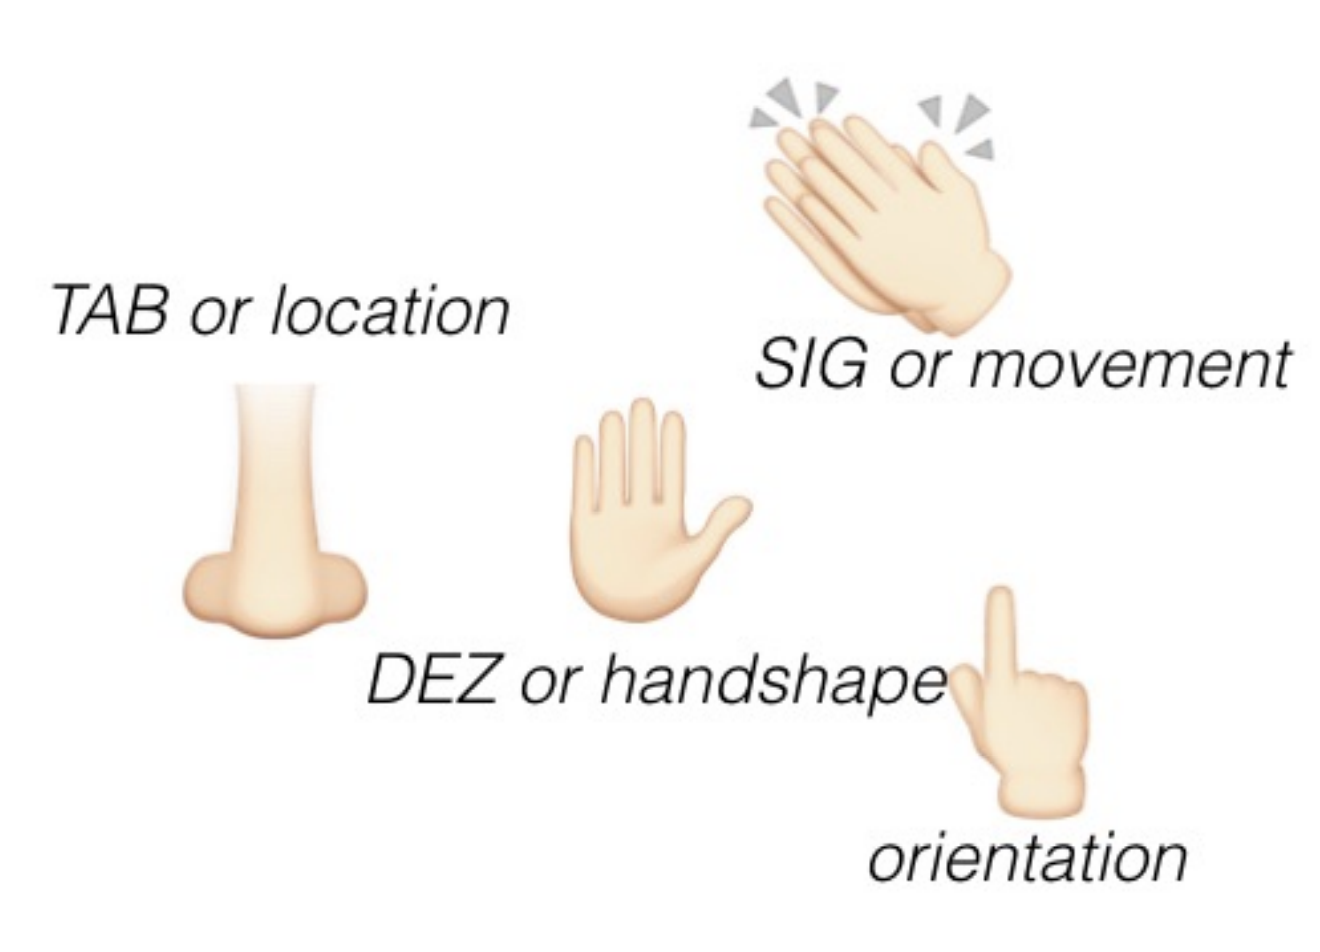
\includegraphics[width = 2.5in]{chapters/background_work/images/stokoe.png}
  \caption{Stoeke Notation}
  \label{fig:stoeke}
\end{figure}

\subsubsection{SignWriting}
\label{ch:background_work:sign_language_descriptions:lexical_approaches:signwriting}

SignWriting is a writing system developed by Valerie Sutton just after DanceWriting~\cite{sutton1973sutton} in the 1970s to represent \gls{sl} visually. It was later included as a part of the MovementWriting system. It is a featural script, representing the features of signs, such as handshapes, movements, and locations. SignWriting is designed to be easy to read and write, with symbols that resemble the gestures they represent. The script is written in two dimensions, with symbols arranged in a grid-like structure to capture various aspects of signs. Figure~\ref{fig:signwriting_coffee} shows an example of how the word "coffee" is represented in SignWriting. SignWriting has been used to transcribe over 40 sign languages worldwide and is recognized by the \gls{iswa} organization.

\begin{figure}
  \centering 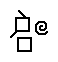
\includegraphics[width = 2.5in]{chapters/background_work/images/signwriting_coffee.png}
  \caption{Coffee in SignWriting}
  \label{fig:signwriting_coffee}
\end{figure}

\subsubsection{HamNoSys}
\label{ch:background_work:sign_language_descriptions:lexical_approaches:hamnosys}

The \gls{hamnosys} is a phonetic transcription system for documenting sign languages globally, developed in 1985 at the University of Hamburg. Unlike Stokoe's notation, which was specifically created for \gls{asl}, HamNoSys aims for broader application, transcending national \gls{hamnosys} boundaries. While Stokoe notation was later adapted to other sign languages, HamNoSys was designed from the outset to accommodate the diversity found in global sign languages.

The notation system employs nearly 200 symbols, organized into five primary categories, each capturing different aspects of a sign. These categories are Handshape, Hand Orientation, Hand Location, Movement, Symmetry Operator, and Non-Manual Markers. To describe a sign, a sequence of symbols is used, with each symbol corresponding to a specific feature. The symbols are arranged in a precise order: first, Handshape, followed by Hand Orientation, Hand Location, Movement, Symmetry Operator, and finally, Non-Manual Markers. This structured sequence allows for a clear and detailed representation of the sign. Figure~\ref{fig:hamnosys_coffee} shows how the word "coffee" is represented in HamNoSys.

HamNoSys offers a detailed representation of the nuanced components in an \gls{sl} \gls{utterance} rather than serving as a practical writing system. Its main purpose is linguistic, used primarily by linguists to analyze the specific features of individual signs. However, it has also found its applications in synthesis~\cite{elliott2010towards} as well as sign detection~\cite{mocialov2022unsupervised}.

\begin{figure}
  \centering 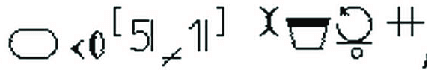
\includegraphics[width = 2.5in]{chapters/background_work/images/hamnosys_coffee.png}
  \caption{Coffee in HamNoSys}
  \label{fig:hamnosys_coffee}
\end{figure}

\subsection{AZee}
\label{ch:background_work:sign_language_descriptions:azee}

Even though these previously discussed lexical approaches are effective in capturing the individual components of signs, they are limited in their ability to represent the dynamic and context-sensitive nature of \gls{sl} discourse. Thus, their appliations in \gls{sl} synthesis are limited. The AZee model however, is grounded in the concept of production rules, which link specific meanings to observable forms. This model operates on the principle that the meaning of a sign can be broken down into a set of features, which are then represented through production rules. These rules guide the generation of the sign's form, encompassing aspects like handshape, movement, and location. Designed to be both flexible and extensible, the AZee model is capable of representing a broad spectrum of signs and sign languages. It is particularly advantageous for \gls{sl} synthesis, offering a systematic and structured method for describing signs and their components.

\subsubsection{Representation of an \gls{utterance} in AZee}
\label{ch:background_work:sign_language_descriptions:azee:representation}

The AZee model uses a hierarchical structure to represent signs, with each level capturing different aspects of the sign. At the lowest level, the model describes the physical form of the sign, such as handshapes, movements, and locations. These physical forms are then combined to create more complex signs, forming a hierarchical structure that mirrors the linguistic structure of the sign. To understand this better, consider the example of the \gls{utterance} "a person aged 52" in \gls{lsf} from the \emph{1R-JP} discourse from the 40 brèves corpus~\cite{challant2022first}. The AZee code for this \gls{utterance} would be:

\begin{verbatim}
  :info-about
    'topic
    :personne
    'info
    :info-about
      'topic
      :âge
      'info
      :tens-units
        'tens
        .nb-5
        'units
        .nb-2
\end{verbatim}

The \gls{azee_interpreter} parses this description recursively, generating an \gls{azee_score}. An \gls{azee_score} being recursive in nature can contain other \gls{azee_score}s. The figure~\ref{fig:azee_score_example} shows the recursive structure for the \gls{utterance} "a person aged 52" using the AZee model. Each of the blocks in the figure represents an \gls{azee_score} .

todo fix diagram with sync rules
\begin{figure}[h]
  \centering 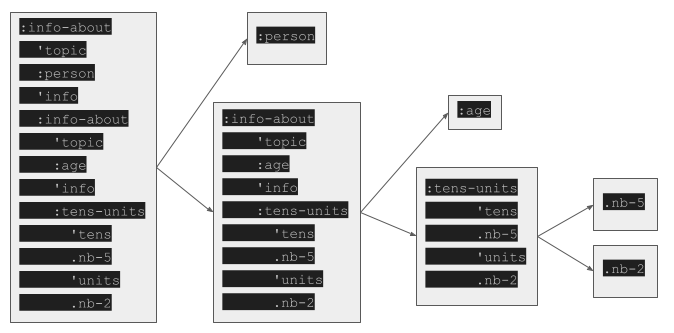
\includegraphics[width = 2.5in]{chapters/background_work/images/azee_score_example.png}
  \caption{AZee's recursive score representation for the \gls{utterance} "a person aged 52"}
  \label{fig:azee_score_example}
\end{figure}

Note that the \gls{score} representation also gives us temporal inforamtion about the \gls{utterance}. Such a detailed representation is important to us as it can help in creation of a timeline and will also be the input for our \gls{sl} synthesis system. 

\subsubsection{Low-Level Descriptions in AZee}
\label{ch:background_work:sign_language_descriptions:azee:low_level}

Apart from the high-level representation of an \gls{utterance} as shown in figure ~\ref{fig:azee_score_example}, the AZee model also supports low-level descriptions that directly correlate with the postures of an abstract avatar. This low-level description is also a recursive \gls{azee_score} and contains a set of \gls{cstr_score}s. A \gls{cstr_score} is a score which contains a set of \gls{posture_constraint}s on the posture that capture various components of the utterance, such as handshapes, movements, and locations. For example, let's consider the \gls{azee_score} for \emph{:personne} (person in \gls{lsf}, figure~\ref{fig:person_lsf}) in the above utterance. Figure ~\ref{fig:azee_score_person} shows the low-level description for this \gls{azee_score}. It contains 4 \gls{cstr_score}s, \emph{HAND\_START}, \emph{HAND\_END}, \emph{HAND\_PATH}, and \emph{PERM}, each containing \gls{posture_constraint}s on the posture of the avatar.

todo create this diagram
\begin{figure}
  \centering 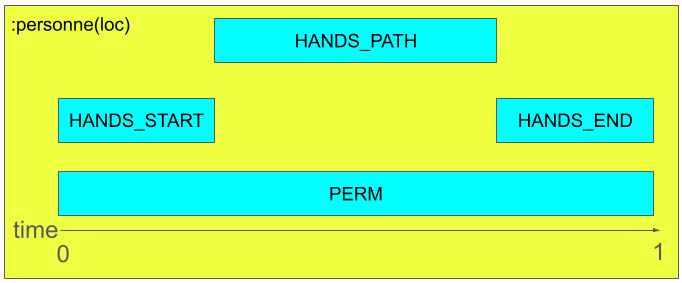
\includegraphics[width = 2.5in]{chapters/background_work/images/azee_score_person.png}
  \caption{Low-level description for the \gls{cstr_score} \emph{:personne}}
  \label{fig:azee_score_person}
\end{figure}

todo add this diagram
\begin{figure}
  \centering 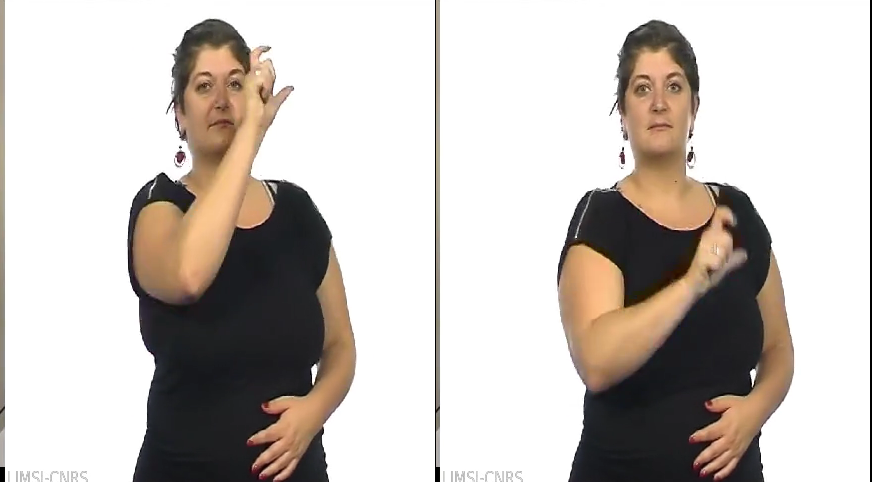
\includegraphics[width = 2.5in]{chapters/background_work/images/person_lsf.png}
  \caption{Person in \gls{lsf}}
  \label{fig:person_lsf}
\end{figure}

\emph{HAND\_START} and \emph{HAND\_END} represent the hands placements and orientations at the start and end of the sign, respectively. \emph{HAND\_PATH} captures the trajectory of the head during the sign, while \emph{PERM} contains the permanent feature such as hand shape.

Finally an \gls{azee_score} can be of various types. These include:

\begin{itemize}
  \item \textbf{Synced Score}: A recrusive structure containing other scores with some relative timing information (figure~\ref{fig:azee_score_example}).
  \item \textbf{\gls{cstr_score}}: A score specifying \gls{posture_constraint}s on the body parts (figure~\ref{fig:azee_score_person}).
  \item \textbf{Hold Score}: A score holding another score for some amount of time.
  \item \textbf{KeyFrame Score}: An abstract \emph{flattened} representation of a \gls{cstr_score}.
  \item \textbf{Non-Animated KeyFrame Score}: A \emph{flattened} representation of \gls{posture_constraint}s on body parts per frame.
  \item \textbf{Animated KeyFrame Score}: A \emph{flattened} representation of pose changes per frame.
\end{itemize}

In addition to these, the AZee model includes several other important operators and concepts that allows to represdent \gls{sl}. Some of these include,

\begin{itemize}
  \item \textbf{Dynamic Points and Paths}: to define moving targets or locations that body parts should follow.
  \item \textbf{Posture structures}: \emph{posture} provides an abstract site and skeleton representation of the human body. A posture can be modified using \gls{posture_constraint}s such as \emph{place}(placement of body parts), \emph{orient}(orientation of bones), and \emph{morph}(morphoogical change in posture).
  \item \textbf{3D math operations}: Various math operations such as vectors, mathematical curves, and transformations are supported in AZee.
  \item \textbf{Partial Application of Operators}: allows for the partial application of an operator to a set of arguments, effectively creating a new operator.
\end{itemize}

Lastly, an AZee description can also be drawn in the form of svg images using AZVD~\cite{filhol2024software}. Figure~\ref{fig:azvd} shows the visual description for the \gls{utterance} "a person aged 52".

\begin{figure}
  \centering 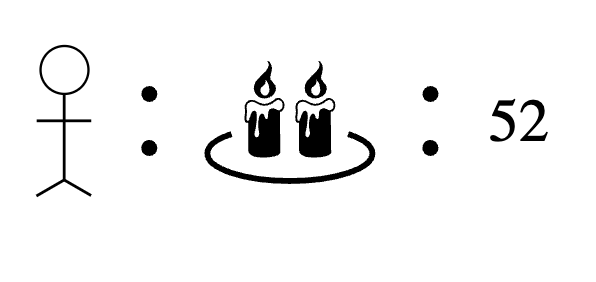
\includegraphics[width = 2.5in]{chapters/background_work/images/azvd.png}
  \caption{AZee visual description for a person aged 52}
  \label{fig:azvd}
\end{figure}

All of these features make the AZee model a powerful tool and a suitable input for our \gls{sl} synthesis system.

\section{\gls{sl} Synthesis}
\label{ch:background_work:sign_language_synthesis}

\gls{sl} synthesis is the process of generating \gls{sl} discourses from linguistic input. This process involves resolving a linguistic description on a digital human. This can be in the form of handshapes, movements, facial expressions, etc. \gls{sl} synthesis is a complex and interdisciplinary field that draws on linguistics, computer science, animation, and human-computer interaction. Several approaches have been developed to synthesize \gls{sl} animations, each with its unique strengths and challenges.

\subsection{2D Techniques}
\label{ch:background_work:sign_language_synthesis:2d_techniques}

Various 2D synthesis~\cite{jiang2024signclipconnectingtextsign, moryossef2024signmtrealtimemultilingualsign} already exist which generate signs directly from \gls{glosses}. One of the newer techniques~\cite{walsh2024sign} addresses the common issue of regression to the mean in previous models, which often resulted in unnatural and under-articulated signing. The authors propose a method called "sign stitching," which involves normalizing signs into a canonical pose, cropping, stitching them together, and applying frequency domain filtering and resampling to produce cohesive, expressive \gls{sl} sequences. They also introduce a Noise Substitution Vector Quantization (NSVQ) transformer to integrate facial expressions, enhancing the naturalness of the signs. The approach is evaluated using a SignGAN model to generate photo-realistic signers, achieving state-of-the-art performance across multiple datasets and receiving positive feedback in user evaluations for its realism and expressiveness. The synthesis is in the form of a 2D video, fitted on the mediapipe a GAN.

Figures~\ref{fig:synthesis_mediaipe_2d} and~\ref{fig:synthesis_gan_2d} illustrate how the output of such methods usually look like, showing the initial mediapipe-based synthesis and the subsequent fitting of a GAN on the Mediapipe skeleton to enhance the realism of the generated signs.

\begin{figure}
  \centering 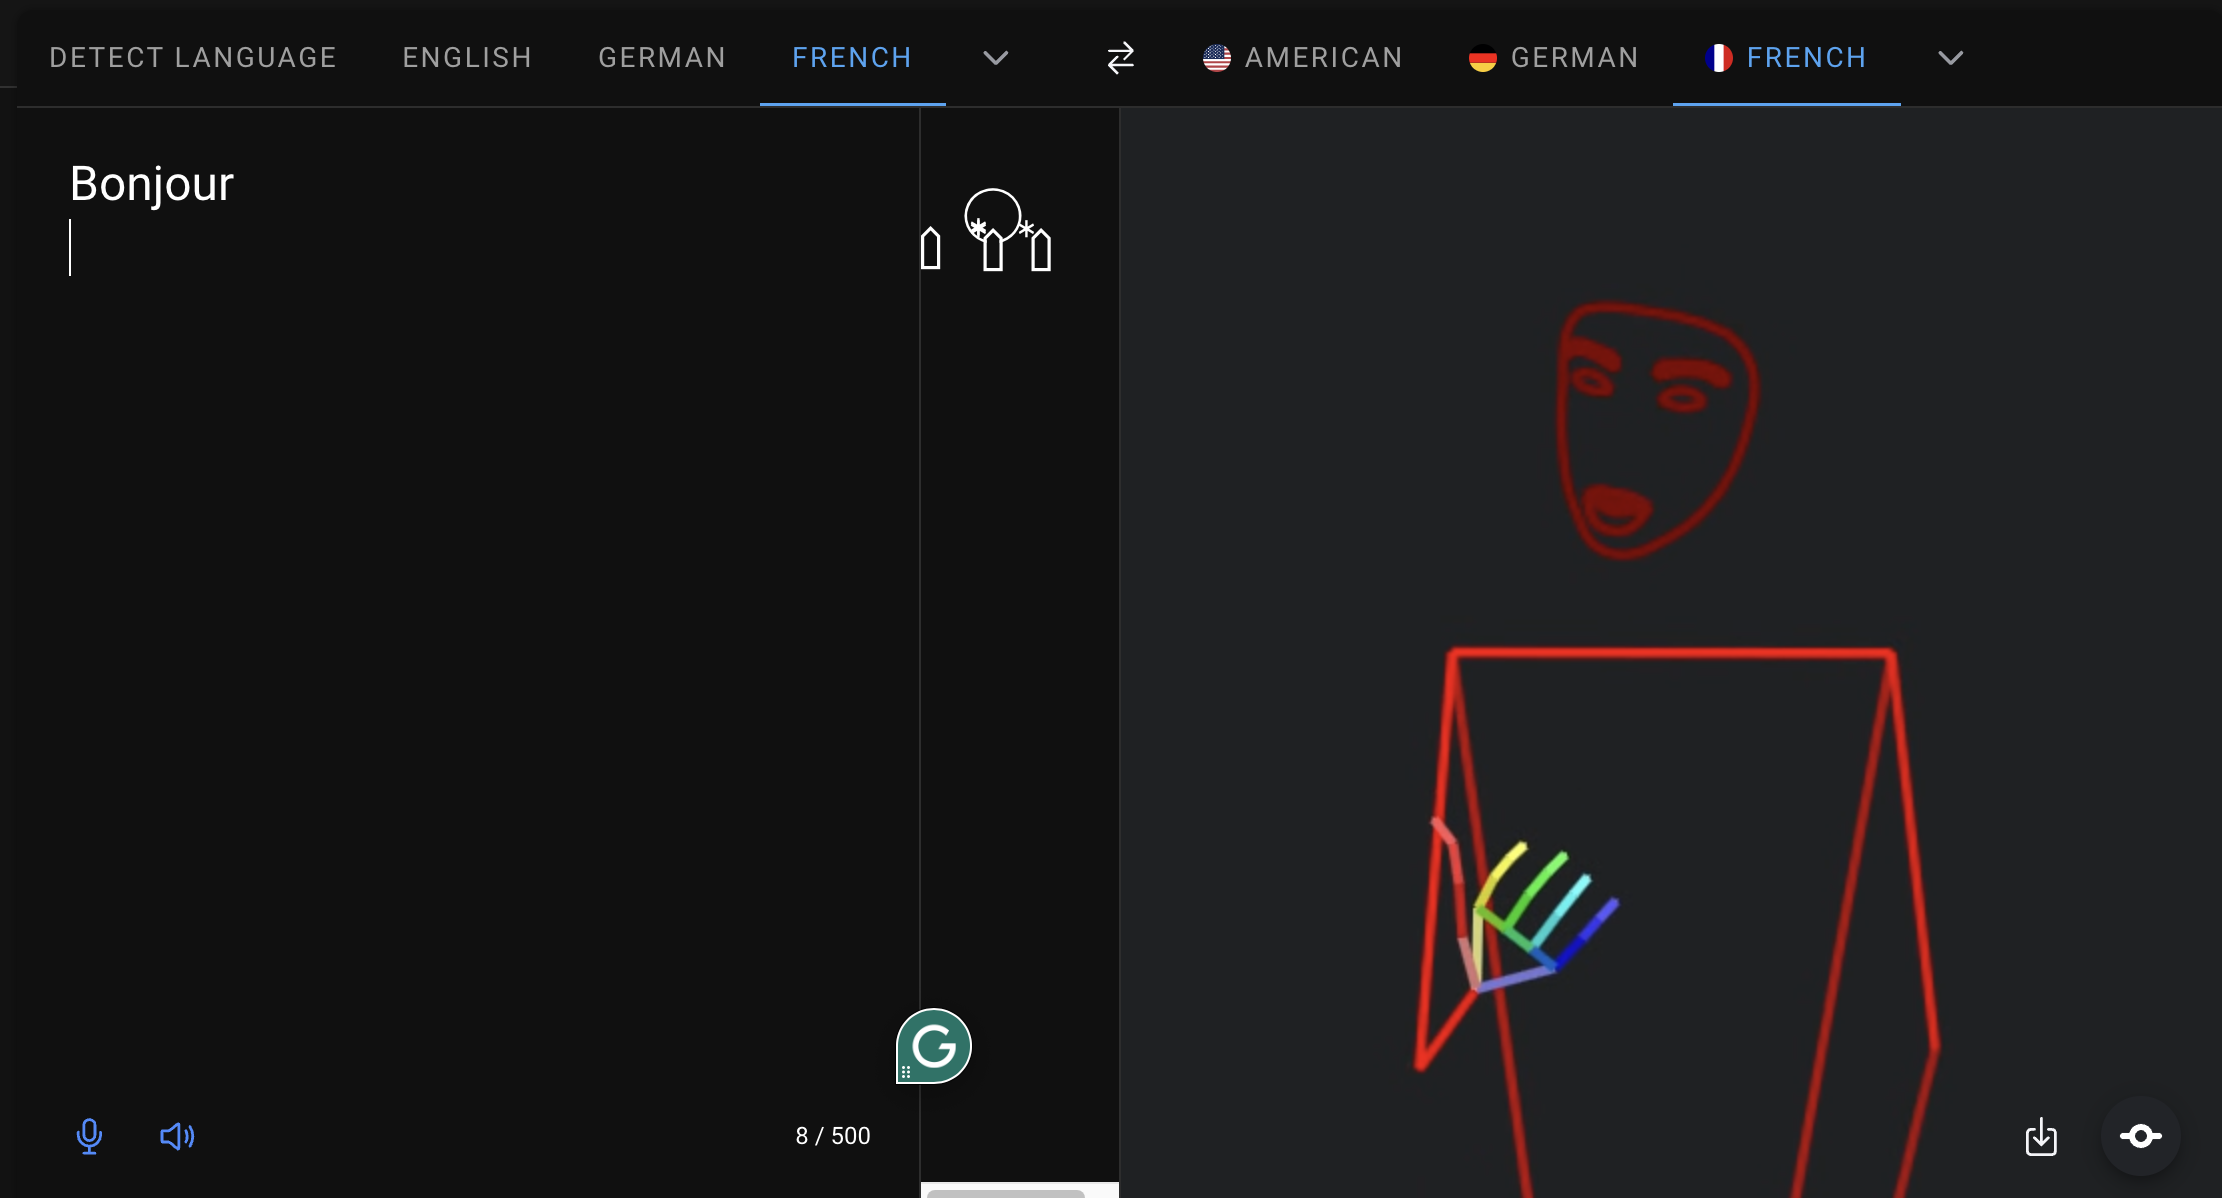
\includegraphics[width = 2.5in]{chapters/background_work/images/sign_writing_synthesis.png} 
  \caption{Synthesis using Sign-Stitching} 
  \label{fig:synthesis_mediaipe_2d} 
\end{figure}

\begin{figure} 
  \centering 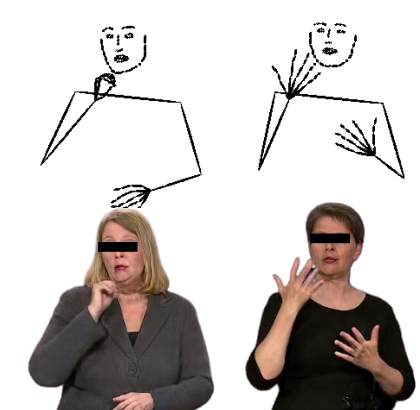
\includegraphics[width = 2.5in]{chapters/background_work/images/gan_synthesis.png} 
  \caption{Fitting a GAN on the Mediapipe skeleton synthesis} 
  \label{fig:synthesis_gan_2d} 
\end{figure}

While such techniques are computationally less demanding, they lack the depth and realism of 3D animations and struggle with capturing complex spatial relationships in Sign Language.

\subsection{3D Techniques}
\label{ch:background_work:sign_language_synthesis:3d_techniques}

3D techniques (albeit being more computationally expensive) generate \gls{sl} animations using avatars that operate in a three-dimensional space. These methods provide a more immersive and realistic representation of SL. 3D synthesis can leverage advanced avatars, such as those created by MetaHuman or SMPL-X, to achieve high levels of detail and expressiveness. Avatars are digital representations of characters or individuals, and are quite poular in in \gls{sl} synthesis to animate the described signs. This subsection explores the components of avatar creation and animation, followed by their use in \gls{sl} synthesis.

\subsubsection{Skeleton}
\label{ch:background_work:sign_language_synthesis:3d_techniques:skeleton}

The skeleton of a digital avatar is a crucial component for enabling realistic movement and animation. It consists of a hierarchical structure of bones, joints, and \gls{posture_constraint}s that mimic the human skeletal system. This section explores several popular skeleton systems used in avatar creation and animation.

\paragraph{Mixamo}
\label{ch:background_work:sign_language_synthesis:3d_techniques:skeleton:mixamo}

Mixamo is a widely used online platform that provides a vast library of pre-rigged 3D characters and animations. Developed by Adobe, Mixamo offers an easy-to-use interface where users can upload their 3D models and automatically rig(add skeleton and other controllable features) them using Mixamo's auto-rigging tool. This tool identifies keypoints on the model and generates a skeleton with appropriate bone placements. Additionally, Mixamo offers a range of pre-made animations that can be applied to the rigged models, facilitating quick and efficient animation workflows. The platform supports various file formats and is compatible with many 3D software tools. A standard Mixamo skeleton consists of 65 bones, covering major body parts, including the spine, arms, legs, hands, and head. Figure~\ref{fig:mixamo_autorigging} shows the process of auto-rigging a 3D model using Mixamo, while Figure~\ref{fig:mixamo_skeleton} illustrates the standard Mixamo skeleton structure.

\begin{figure} 
  \centering 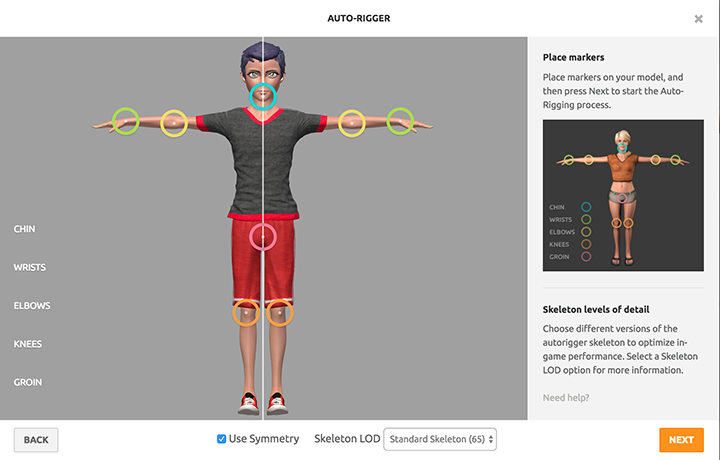
\includegraphics[width = 2.5in]{chapters/background_work/images/mixamo_autorigging.png} 
  \caption{Autorigging using Mixamo} 
  \label{fig:mixamo_autorigging} 
\end{figure}

\begin{figure} 
  \centering 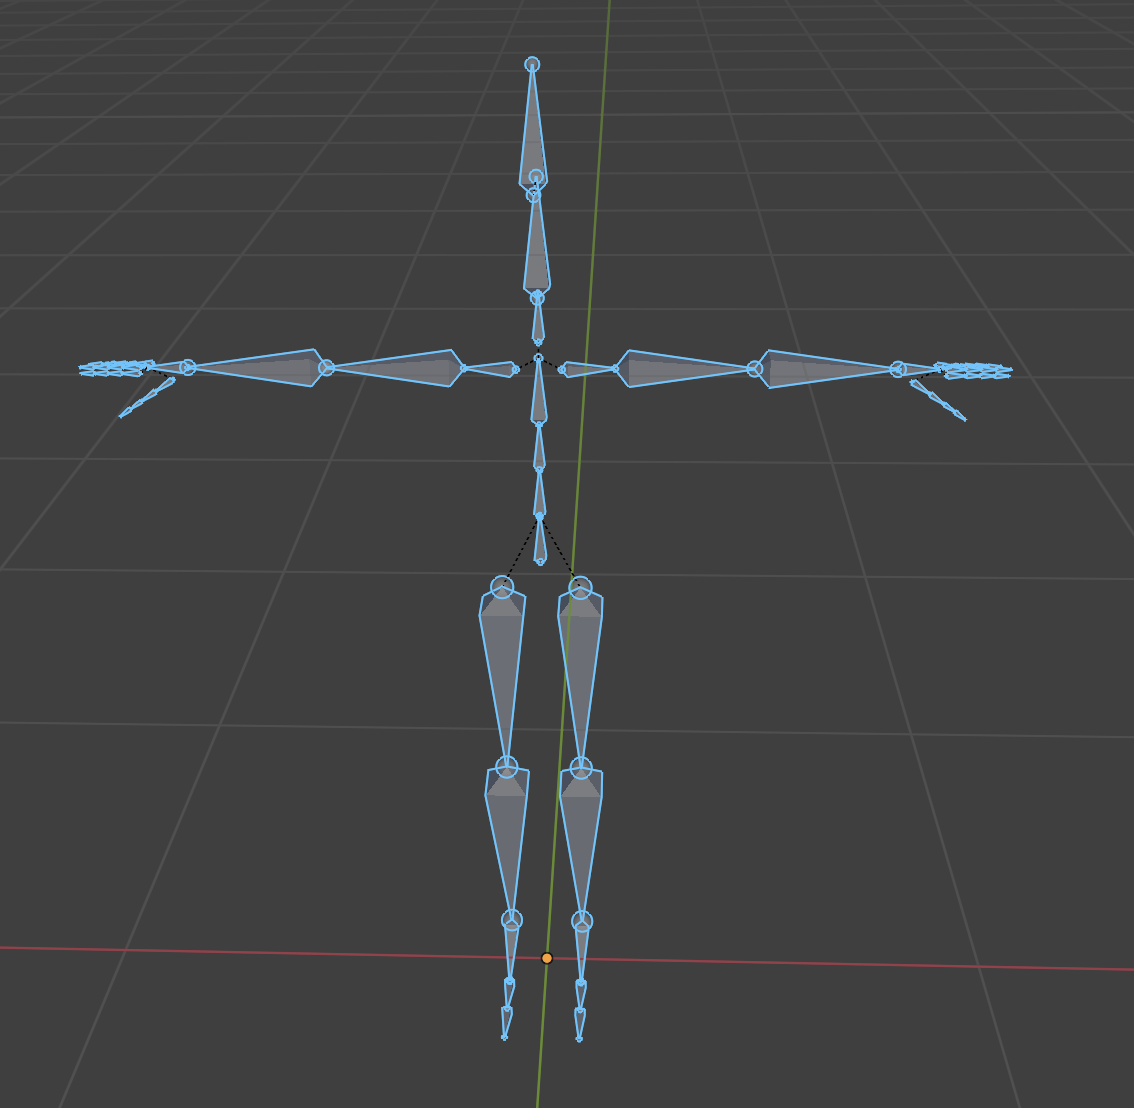
\includegraphics[width = 2.5in]{chapters/background_work/images/mixamo_skeleton.png} 
  \caption{Standard Mixamo skeleton structure} 
  \label{fig:mixamo_skeleton} 
\end{figure}

\paragraph{SMPL-X}
\label{ch:background_work:sign_language_synthesis:3d_techniques:skeleton:smpl_x}

SMPL-X (Skinned Multi-Person Linear Model eXtended) is a state-of-the-art parametric model for generating highly detailed and anatomically accurate 3D human avatars. SMPL-X encodes the shape and pose of a character using a low-dimensional space, allowing for efficient representation and manipulation. Thus, a configuration of about 100 numbers can represent the pose as well as the shape of the avatar. The hierarchy of a SMPL-X skeleton is shown in figure~\ref{fig:smpl_x_skeleton}, and the corresponding latent space representation in figure~\ref{fig:latent_space_smplx}.

\begin{figure} 
  \centering 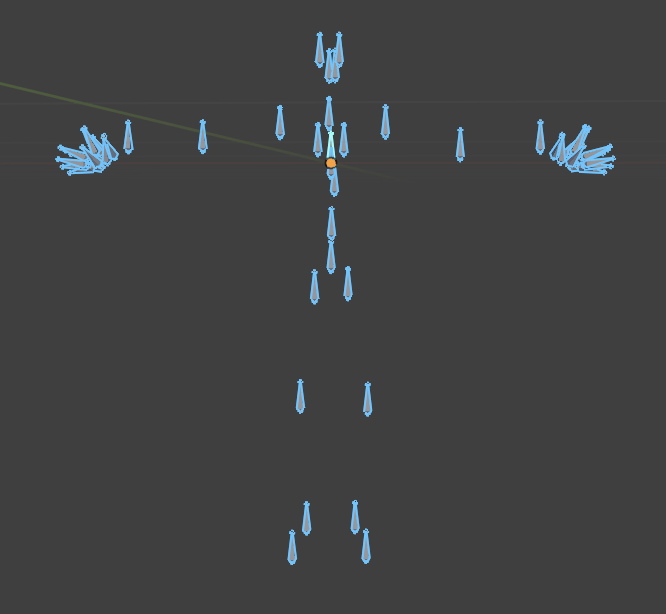
\includegraphics[width = 2.5in]{chapters/background_work/images/smpl_x_skeleton.png} 
  \caption{SMPL-X skeleton} 
  \label{fig:smpl_x_skeleton} 
\end{figure}

\begin{figure} 
  \centering 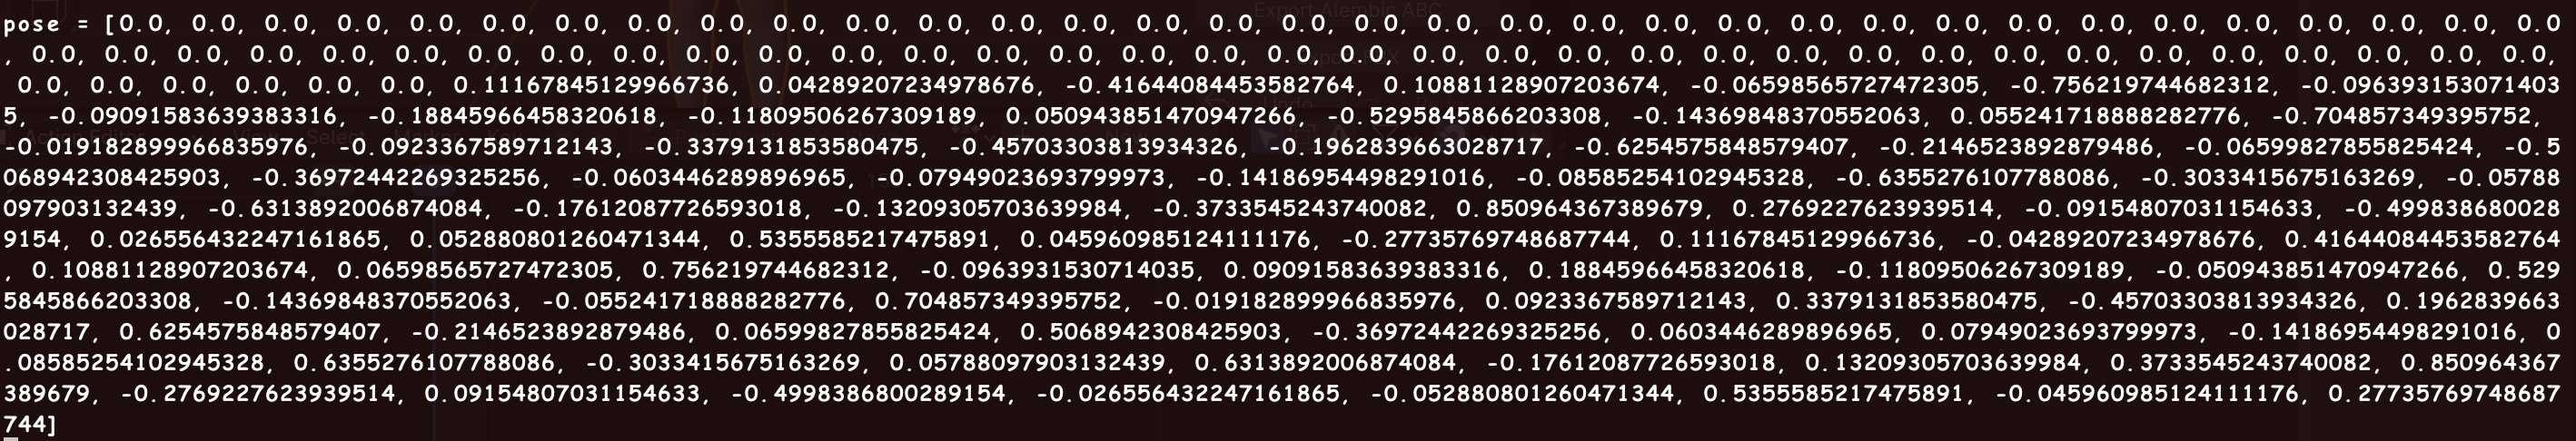
\includegraphics[width = 2.5in]{chapters/background_work/images/latent_space_smplx.png} 
  \caption{SMPL-X latent space} 
  \label{fig:latent_space_smplx} 
\end{figure}

\subsubsection{Mesh and Texture}
\label{ch:background_work:sign_language_synthesis:3d_techniques:mesh_and_texture}

The mesh of a digital avatar is the 3D model that forms the surface representation of the character. It consists of vertices, edges, and faces that define the shape and structure of the avatar. Creating and manipulating meshes is a fundamental aspect of 3D modeling and animation, allowing for detailed and realistic character designs.

Textures are 2D images applied to the surface of a 3D model to enhance its appearance and realism. Textures can represent various surface properties such as color, roughness, reflectivity, and transparency. Common types of textures include diffuse maps (color), specular maps (reflectivity), normal maps (surface detail), and roughness maps (surface smoothness). By combining different textures, artists can create visually compelling avatars with intricate surface details and lifelike appearances. These textures are often mapped onto the mesh of the avatar using UV mapping techniques to ensure proper alignment and scaling.

\paragraph{Weight Painting}
\label{ch:background_work:sign_language_synthesis:3d_techniques:mesh_and_texture:weight_painting}

Weight painting is a technique used to define how much influence each bone in a skeleton has over the surrounding mesh vertices. It plays a crucial role in ensuring that the mesh deforms naturally and realistically when the skeleton is animated. Figure~\ref{fig:weight_painting} shows an example of weight painting in Blender, with the red color indicating high influence and blue indicating low influence.

\begin{figure} 
  \centering 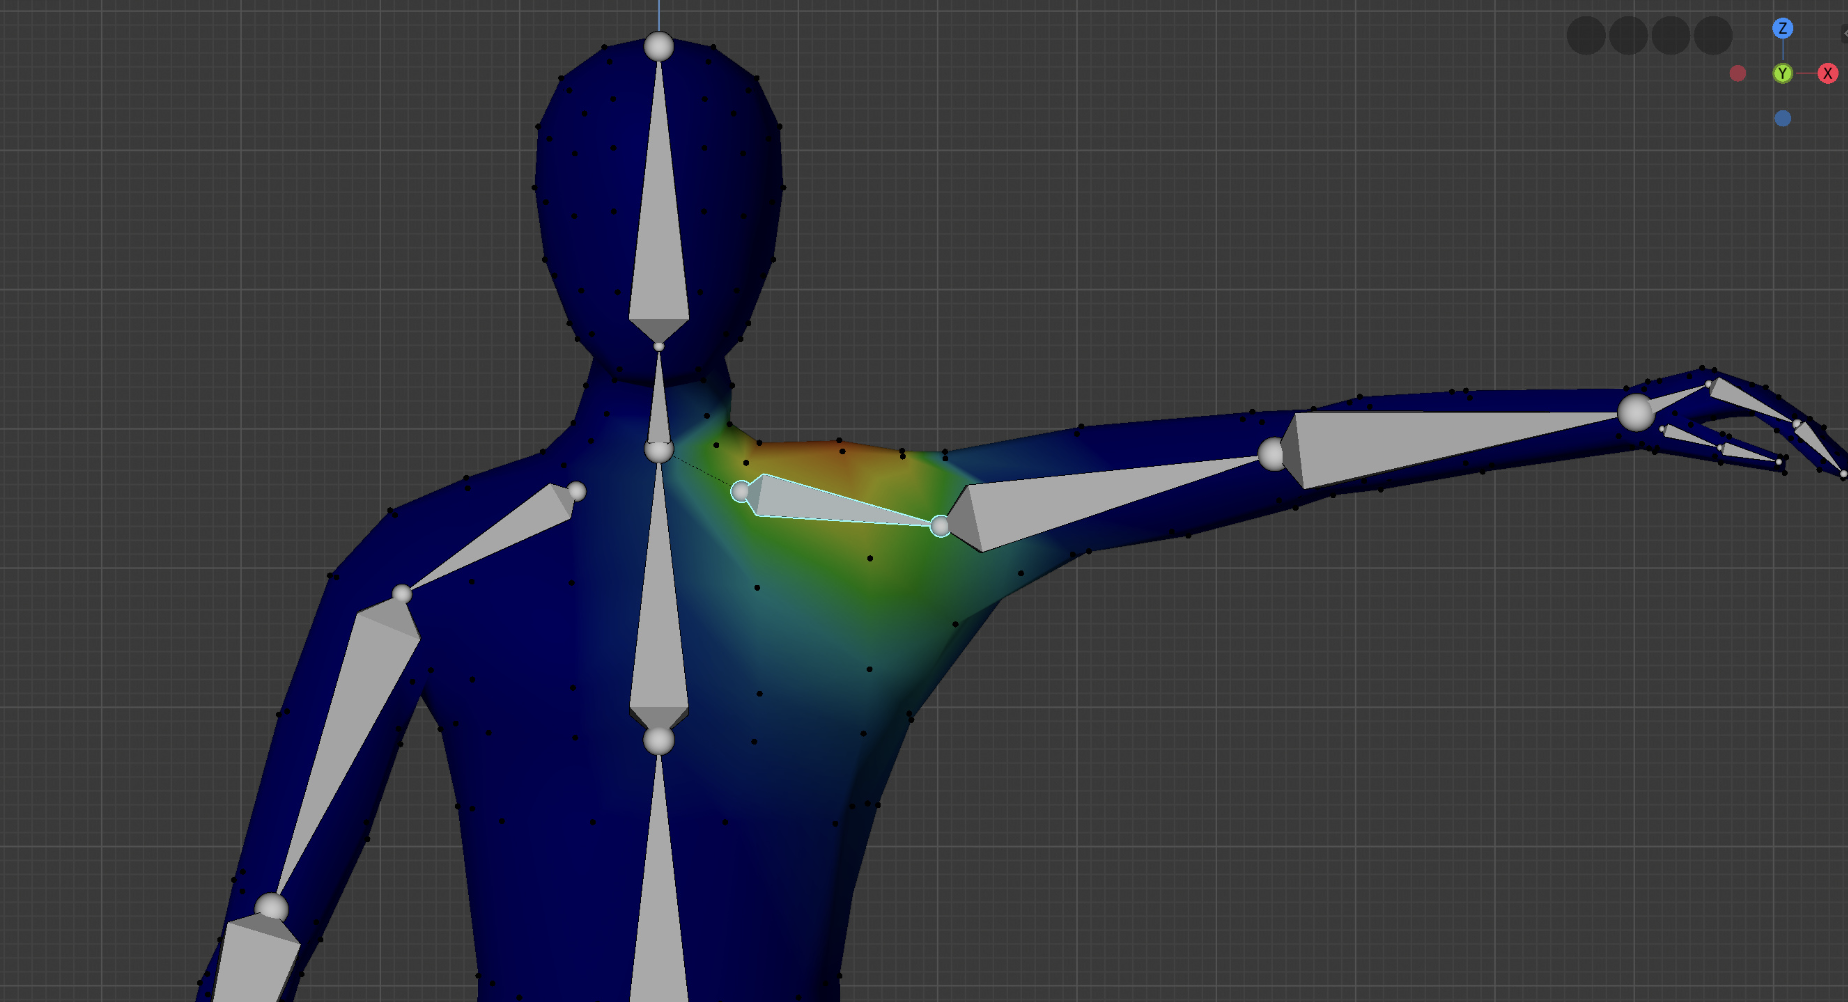
\includegraphics[width = 2.5in]{chapters/background_work/images/weight_painting.png} 
  \caption{Weight painting in Blender} 
  \label{fig:weight_painting} 
\end{figure}

\paragraph{Face Animation: Blend Shapes vs. Bones}
\label{ch:background_work:sign_language_synthesis:3d_techniques:mesh_and_texture:face_animation_blend_shapes_vs_bones}

Modeling and animating the face of an avatar is a complex task that involves creating detailed meshes and intricate animation controls to capture expressions and movements accurately. Blend shapes are used to create different facial expressions by interpolating between multiple versions of a mesh. This technique allows animators to blend between various expressions smoothly, such as smiling, frowning, or blinking. Adding bones to the facial mesh allows for more granular control over facial movements. Each bone can control different parts of the face, such as the jaw, eyebrows, and eyelids. This method is often used in conjunction with blend shapes to enhance expressiveness.

\textbf{Pros and Cons}:

\begin{itemize}
  \item \textbf{Blend Shapes}: Ideal for detailed and smooth transitions between expressions, but limited in flexibility.
  \item \textbf{Bones}: Provide granular control, better for interactive or dynamic facial animations but are more complex to set up and manage.
\end{itemize}

The process of animating facial expressions using blend shapes is shown in figure~\ref{fig:blendshapes_smile}, where the progression of a smile is depicted from 0 to 1.0. Figure~\ref{fig:facial_bones} illustrates the use of facial bones for animating specific areas like the eyes, jaw, and tongue.

\begin{figure}[h]
  \centering
  \begin{subfigure}{0.3\linewidth} 
      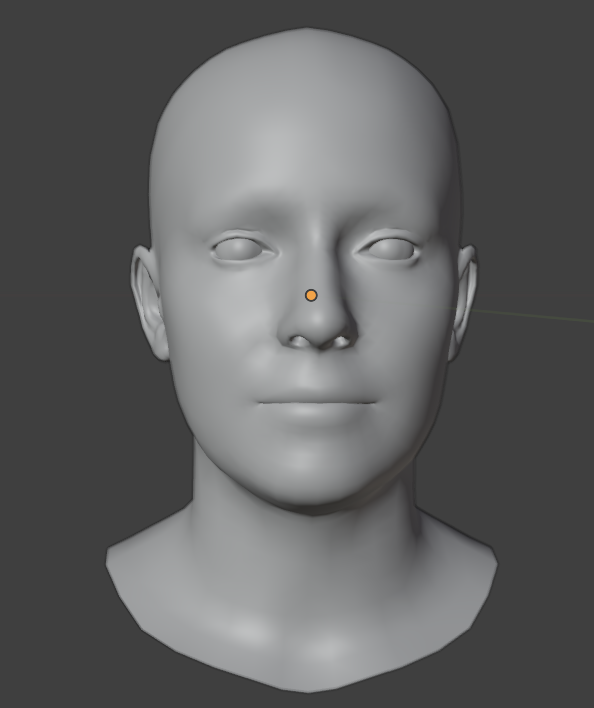
\includegraphics[width=\linewidth]{chapters/background_work/images/blendshapes_example/blendshapes_example_1.png} 
      \caption{Smile at 0} 
  \end{subfigure} 
  \hfill 
  \begin{subfigure}{0.3\linewidth} 
      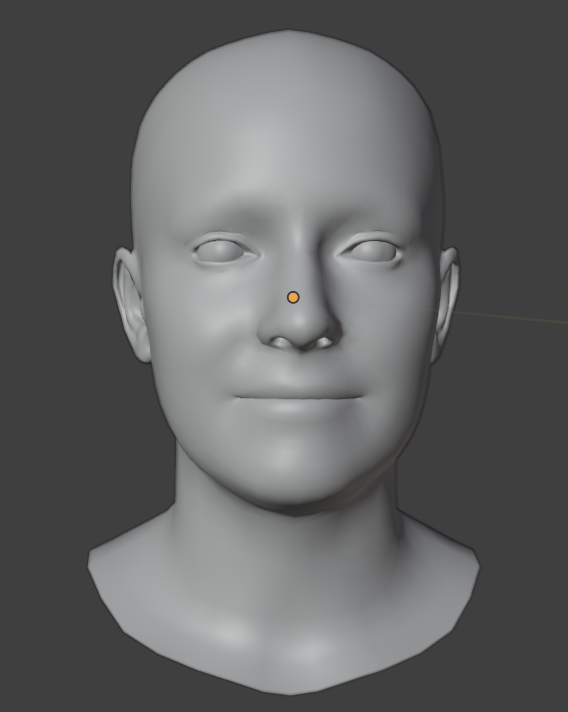
\includegraphics[width=\linewidth]{chapters/background_work/images/blendshapes_example/blendshapes_example_2.png} 
      \caption{Smile at 0.5} 
  \end{subfigure} 
  \hfill 
  \begin{subfigure}{0.3\linewidth} 
      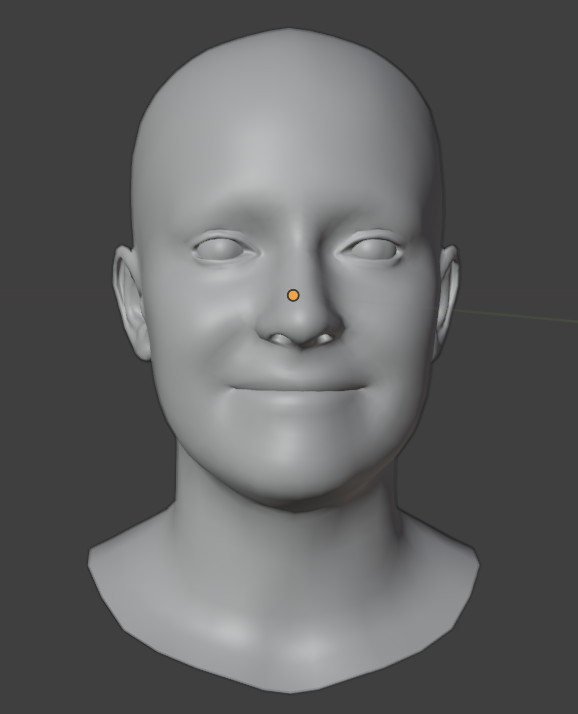
\includegraphics[width=\linewidth]{chapters/background_work/images/blendshapes_example/blendshapes_example_3.png} 
      \caption{Smile at 1} 
  \end{subfigure}
  \caption{Progression of smile using blend shapes from 0 to 1.0}
  \label{fig:blendshapes_smile}
\end{figure}

\begin{figure} 
  \centering 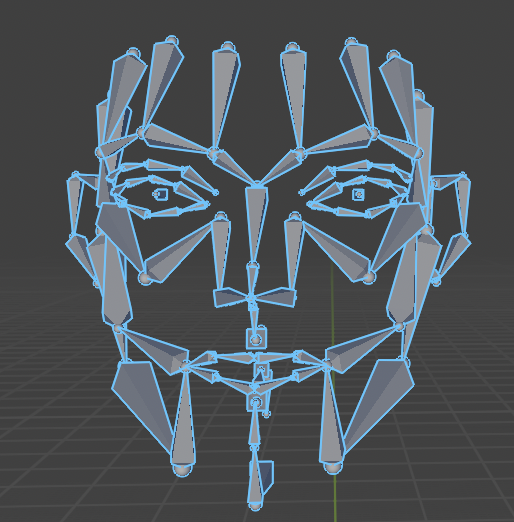
\includegraphics[width = 2.5in]{chapters/background_work/images/facial_bones.png} 
  \caption{Facial bones for eyes, jaw, and tongue} 
  \label{fig:facial_bones} 
\end{figure}

\subsubsection{Rigging}
\label{ch:background_work:sign_language_synthesis:3d_techniques:rigging}

A rig is the final system used by the artists to animate the avatars. This is done by implementing all the above systems in order, i.e., creating a skeleton, mesh, texture, weight painting, facial blend shapes, implementing IK and FK systems, and adding constraints. Figure~\ref{fig:rig_example} shows an example of a rigged character, the "Rain rig" by Blender Studio.

\begin{figure} 
  \centering 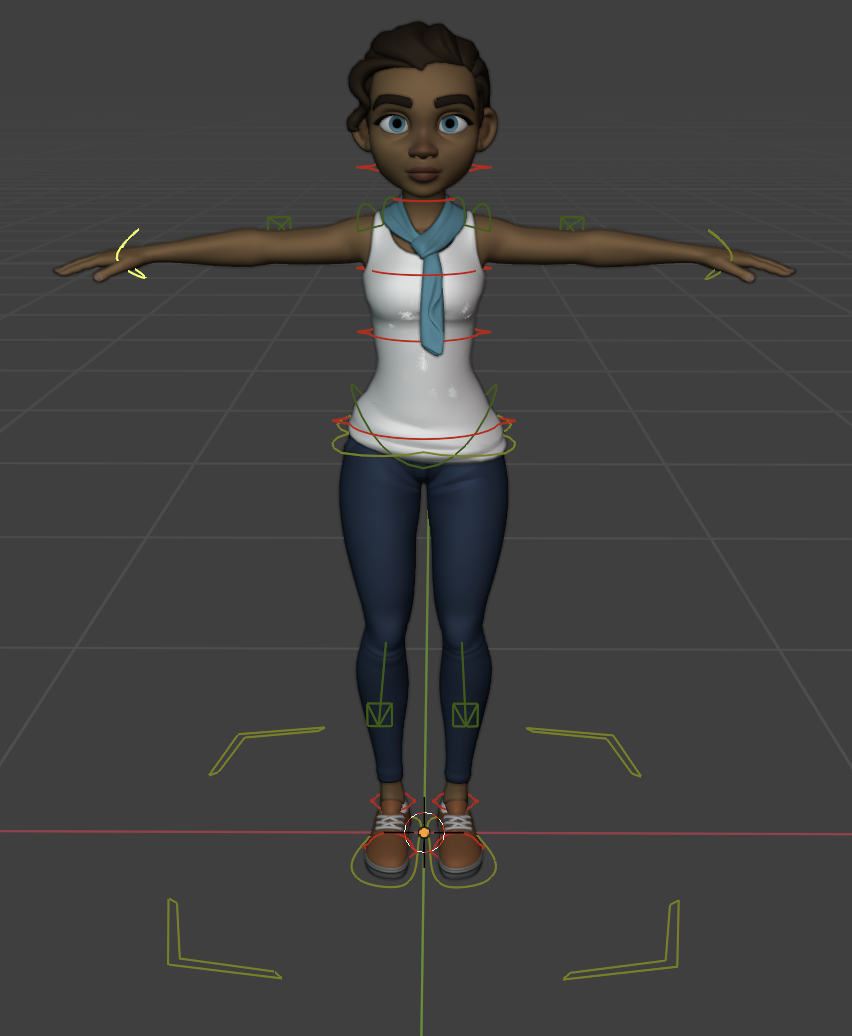
\includegraphics[width = 2.5in]{chapters/background_work/images/rig_example.png} 
  \caption{Rain rig by Blender studio} 
  \label{fig:rig_example} 
\end{figure}

\subsubsection{Procedural Avatar Creation}
\label{ch:background_work:sign_language_synthesis:3d_techniques:procedural_avatar_creation}

Procedural avatar creation involves the use of algorithms and software tools to automatically generate 3D characters with minimal manual intervention. This approach can significantly speed up the character creation process since it automates the creation of all of the avatar components discussed above. This allows rapid development of detailed and diverse avatars. This section explores several prominent tools and models used for procedural avatar creation.

\paragraph{MakeHuman}
\label{ch:background_work:sign_language_synthesis:3d_techniques:procedural_avatar_creation:makehuman}

MakeHuman is an open-source tool specifically designed for the rapid prototyping of humanoid avatars. It allows users to create 3D human models through an intuitive interface where parameters such as gender, age, ethnicity, and body proportions can be adjusted using sliders. Figure~\ref{fig:makehuman_example} demonstrates the process of creating an avatar using MakeHuman.

\begin{figure} 
  \centering 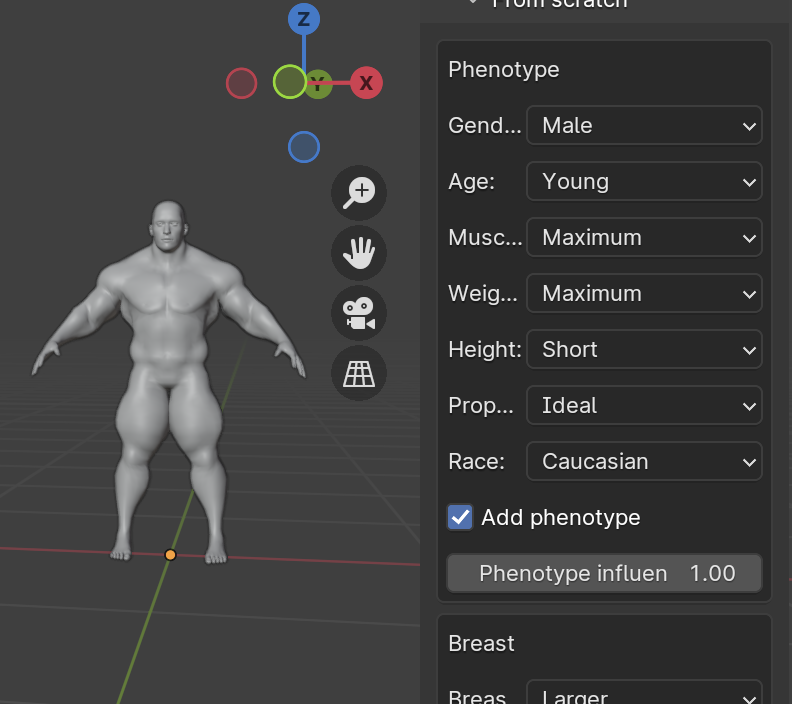
\includegraphics[width = 2.5in]{chapters/background_work/images/makehuman_example.png} 
  \caption{Avatar creation using MakeHuman} 
  \label{fig:makehuman_example} 
\end{figure}

\paragraph{SMPL-X or Meshcapade}
\label{ch:background_work:sign_language_synthesis:3d_techniques:procedural_avatar_creation:smpl_x_meshcapade}

Just like MakeHuman, SMPL-X can create avatars with parameters such as weight, height, age, etc. However, SMPL-X can also be created using images of a person. This allows it to be more realistic than MakeHuman. Figure~\ref{fig:smpl_creation_example} shows the process of creating an SMPL-X avatar using the Meshcapade tool.

\begin{figure} 
  \centering 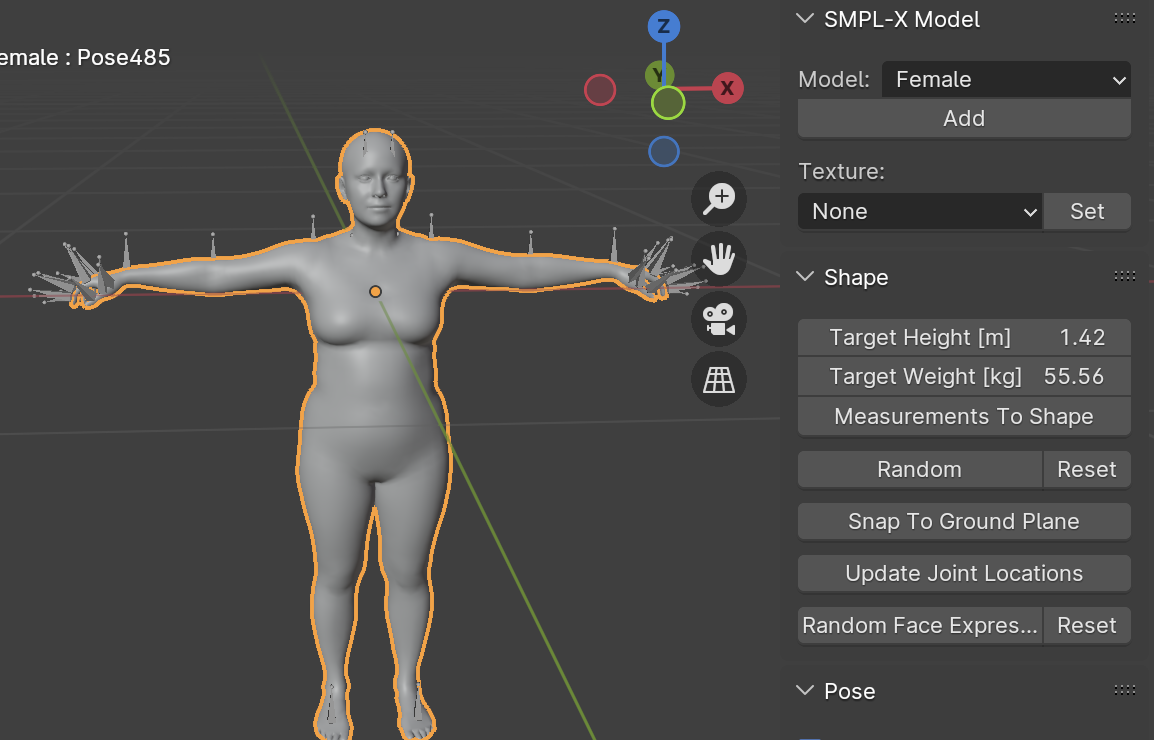
\includegraphics[width = 2.5in]{chapters/background_work/images/smpl_creation_example.png} 
  \caption{SMPL-X avatar creation using Meshcapade} 
  \label{fig:smpl_creation_example} 
\end{figure}

\paragraph{MetaHuman}
\label{ch:background_work:sign_language_synthesis:3d_techniques:procedural_avatar_creation:metahuman}

MetaHuman Creator (figure~\ref{fig:metahuman_example}), developed by Epic Games, is a tool for creating ultra-realistic digital humans. The tool's emphasis on realism and detail makes it a powerful resource for creating lifelike characters for games, films, and other interactive experiences. MetaHumans are the most realistic avatars available today, with high-quality textures, detailed facial expressions, and advanced animation controls.

\begin{figure} 
  \centering 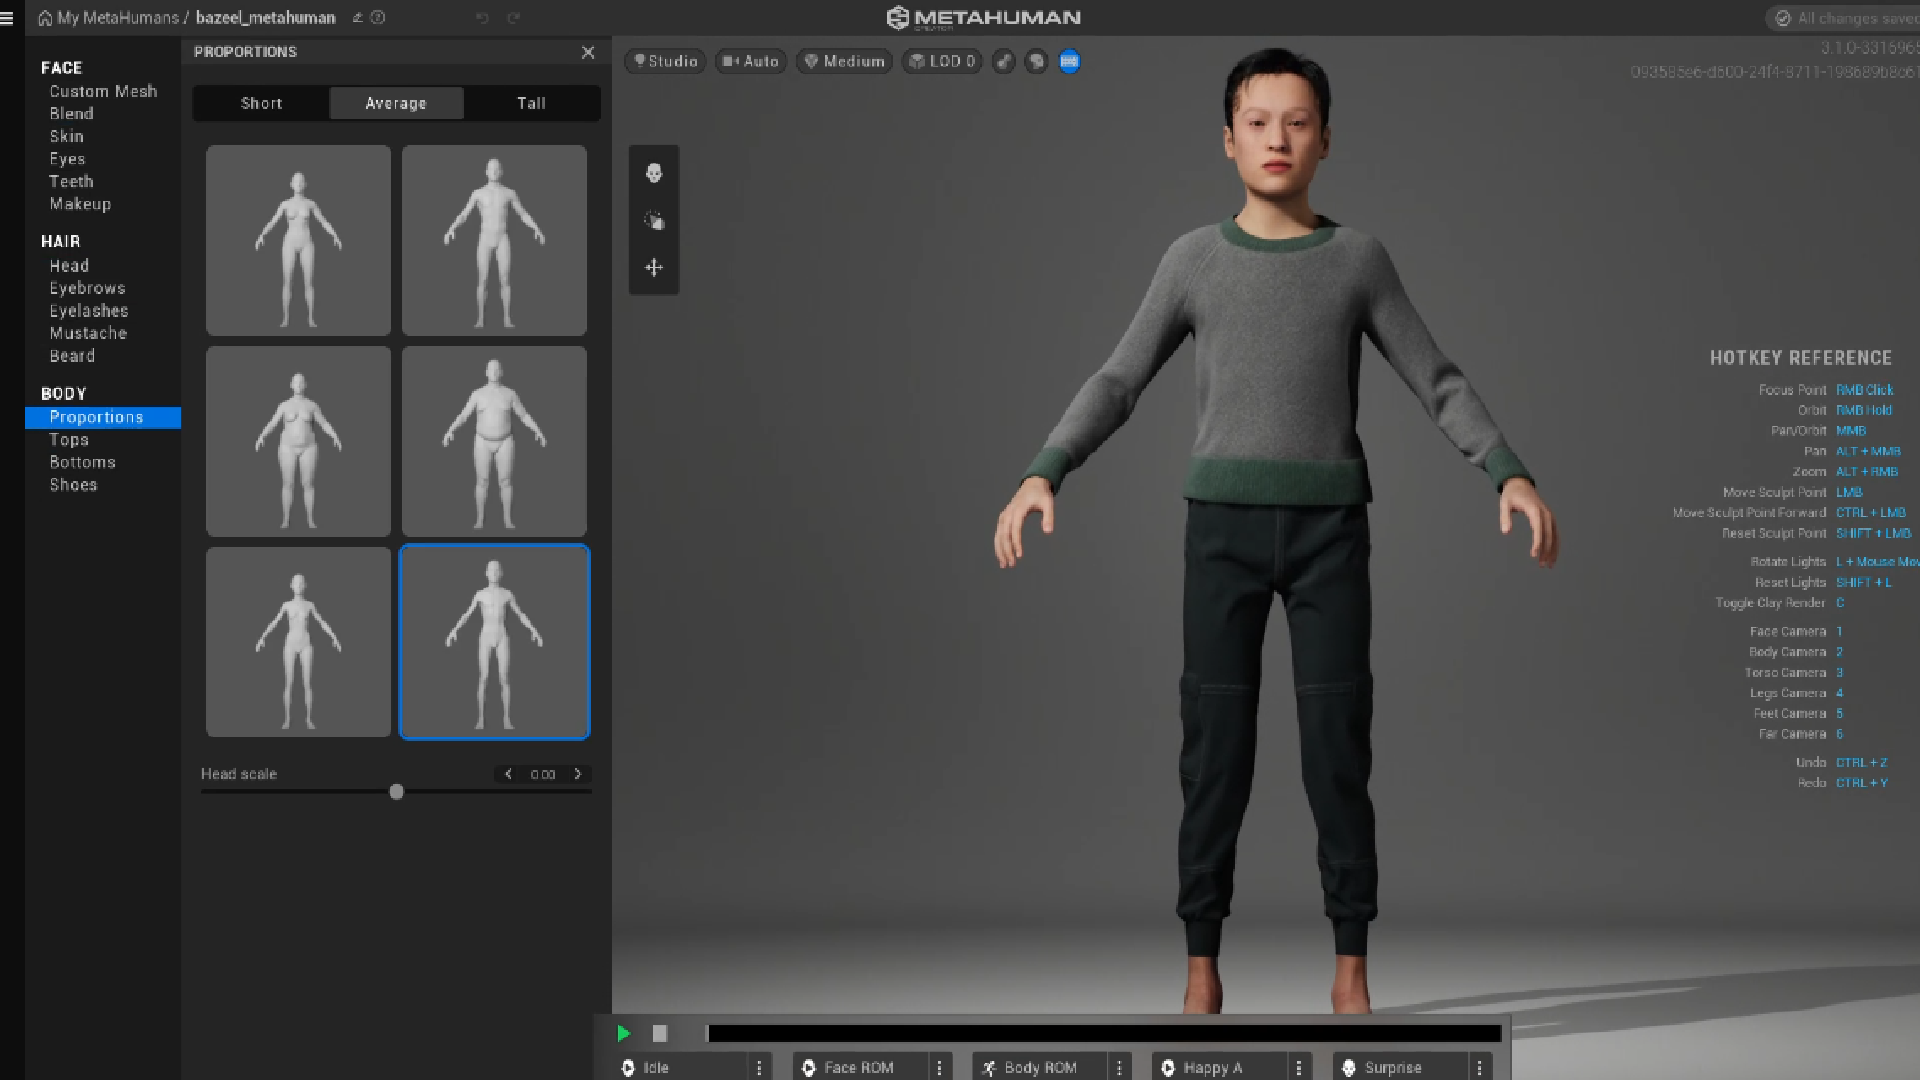
\includegraphics[width = 2.5in]{chapters/background_work/images/metahuman_example.png} 
  \caption{Avatar creation using MetaHuman} 
  \label{fig:metahuman_example}
\end{figure}

\subsubsection{Avatar Animation}
\label{ch:background_work:sign_language_synthesis:3d_techniques:avatar_animation}

The methods used for animating avatars range from manual to automated processes, each offering unique benefits and challenges. This section explores the key methods used in avatar animation.

\paragraph{Manual Keyframing}
\label{ch:background_work:sign_language_synthesis:3d_techniques:avatar_animation:manual_keyframing}

Manual keyframing is a traditional animation technique where animators define specific poses, known as keyframes, at critical points in time. These keyframes mark the start and end points of any smooth transition or movement. The intermediate poses are then calculated using interpolation. This method provides animators with precise control over every aspect of the avatar’s movement, making it ideal for achieving nuanced and detailed animations.

Figure~\ref{fig:keyframing} shows the process of manual keyframing to animate a sprite.

\begin{figure} 
  \centering \includegraphics[width = 2.5in]{chapters/background_work/images/keyframing.png} 
  \caption{Manual keyframing to animate a sprite} 
  \label{fig:keyframing} 
\end{figure}

Along with keyframing, motion curves~\cite{10.1145/218380.218422} are used to control the interpolation between keyframes. These curves define the speed and timing of the animation, allowing animators to create smooth and natural movements. Common types of motion curves include linear, ease-in, ease-out, and bezier curves. By adjusting the shape and slope of these curves, animators can fine-tune the animation to achieve the desired effect. Figure~\ref{fig:motion_curves} shows examples of different motion curves used to fine-tune an animation.

\begin{figure} 
  \centering 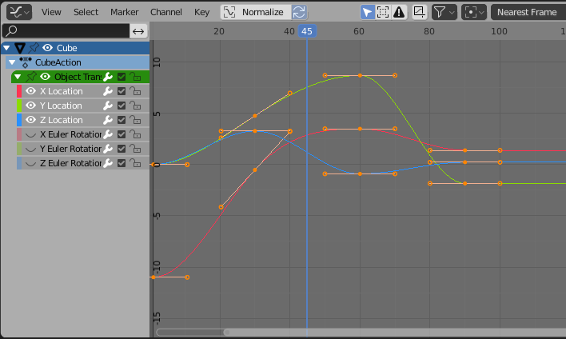
\includegraphics[width = 2.5in]{chapters/background_work/images/motion_curves.png} 
  \caption{Motion curves to finetune an animation} 
  \label{fig:motion_curves} 
\end{figure}

\paragraph{Mocap Retargeting}
\label{ch:background_work:sign_language_synthesis:3d_techniques:avatar_animation:mocap_retargeting}

Motion capture (mocap) retargeting involves capturing the movements of a real human actor and applying this data to a digital avatar. This process starts with recording an actor’s performance using a motion capture system, which tracks the actor’s movements through markers or sensors placed on their body. The recorded data is then mapped onto the avatar’s skeleton, a process known as retargeting. Mocap retargeting ensures highly realistic animations by directly transferring the nuances of human motion to the digital character. This technique is widely used in the entertainment industry, particularly in video games and films, to create lifelike animations.

Figure~\ref{fig:mocap} illustrates the process of motion capture and retargeting.

\begin{figure} 
  \centering 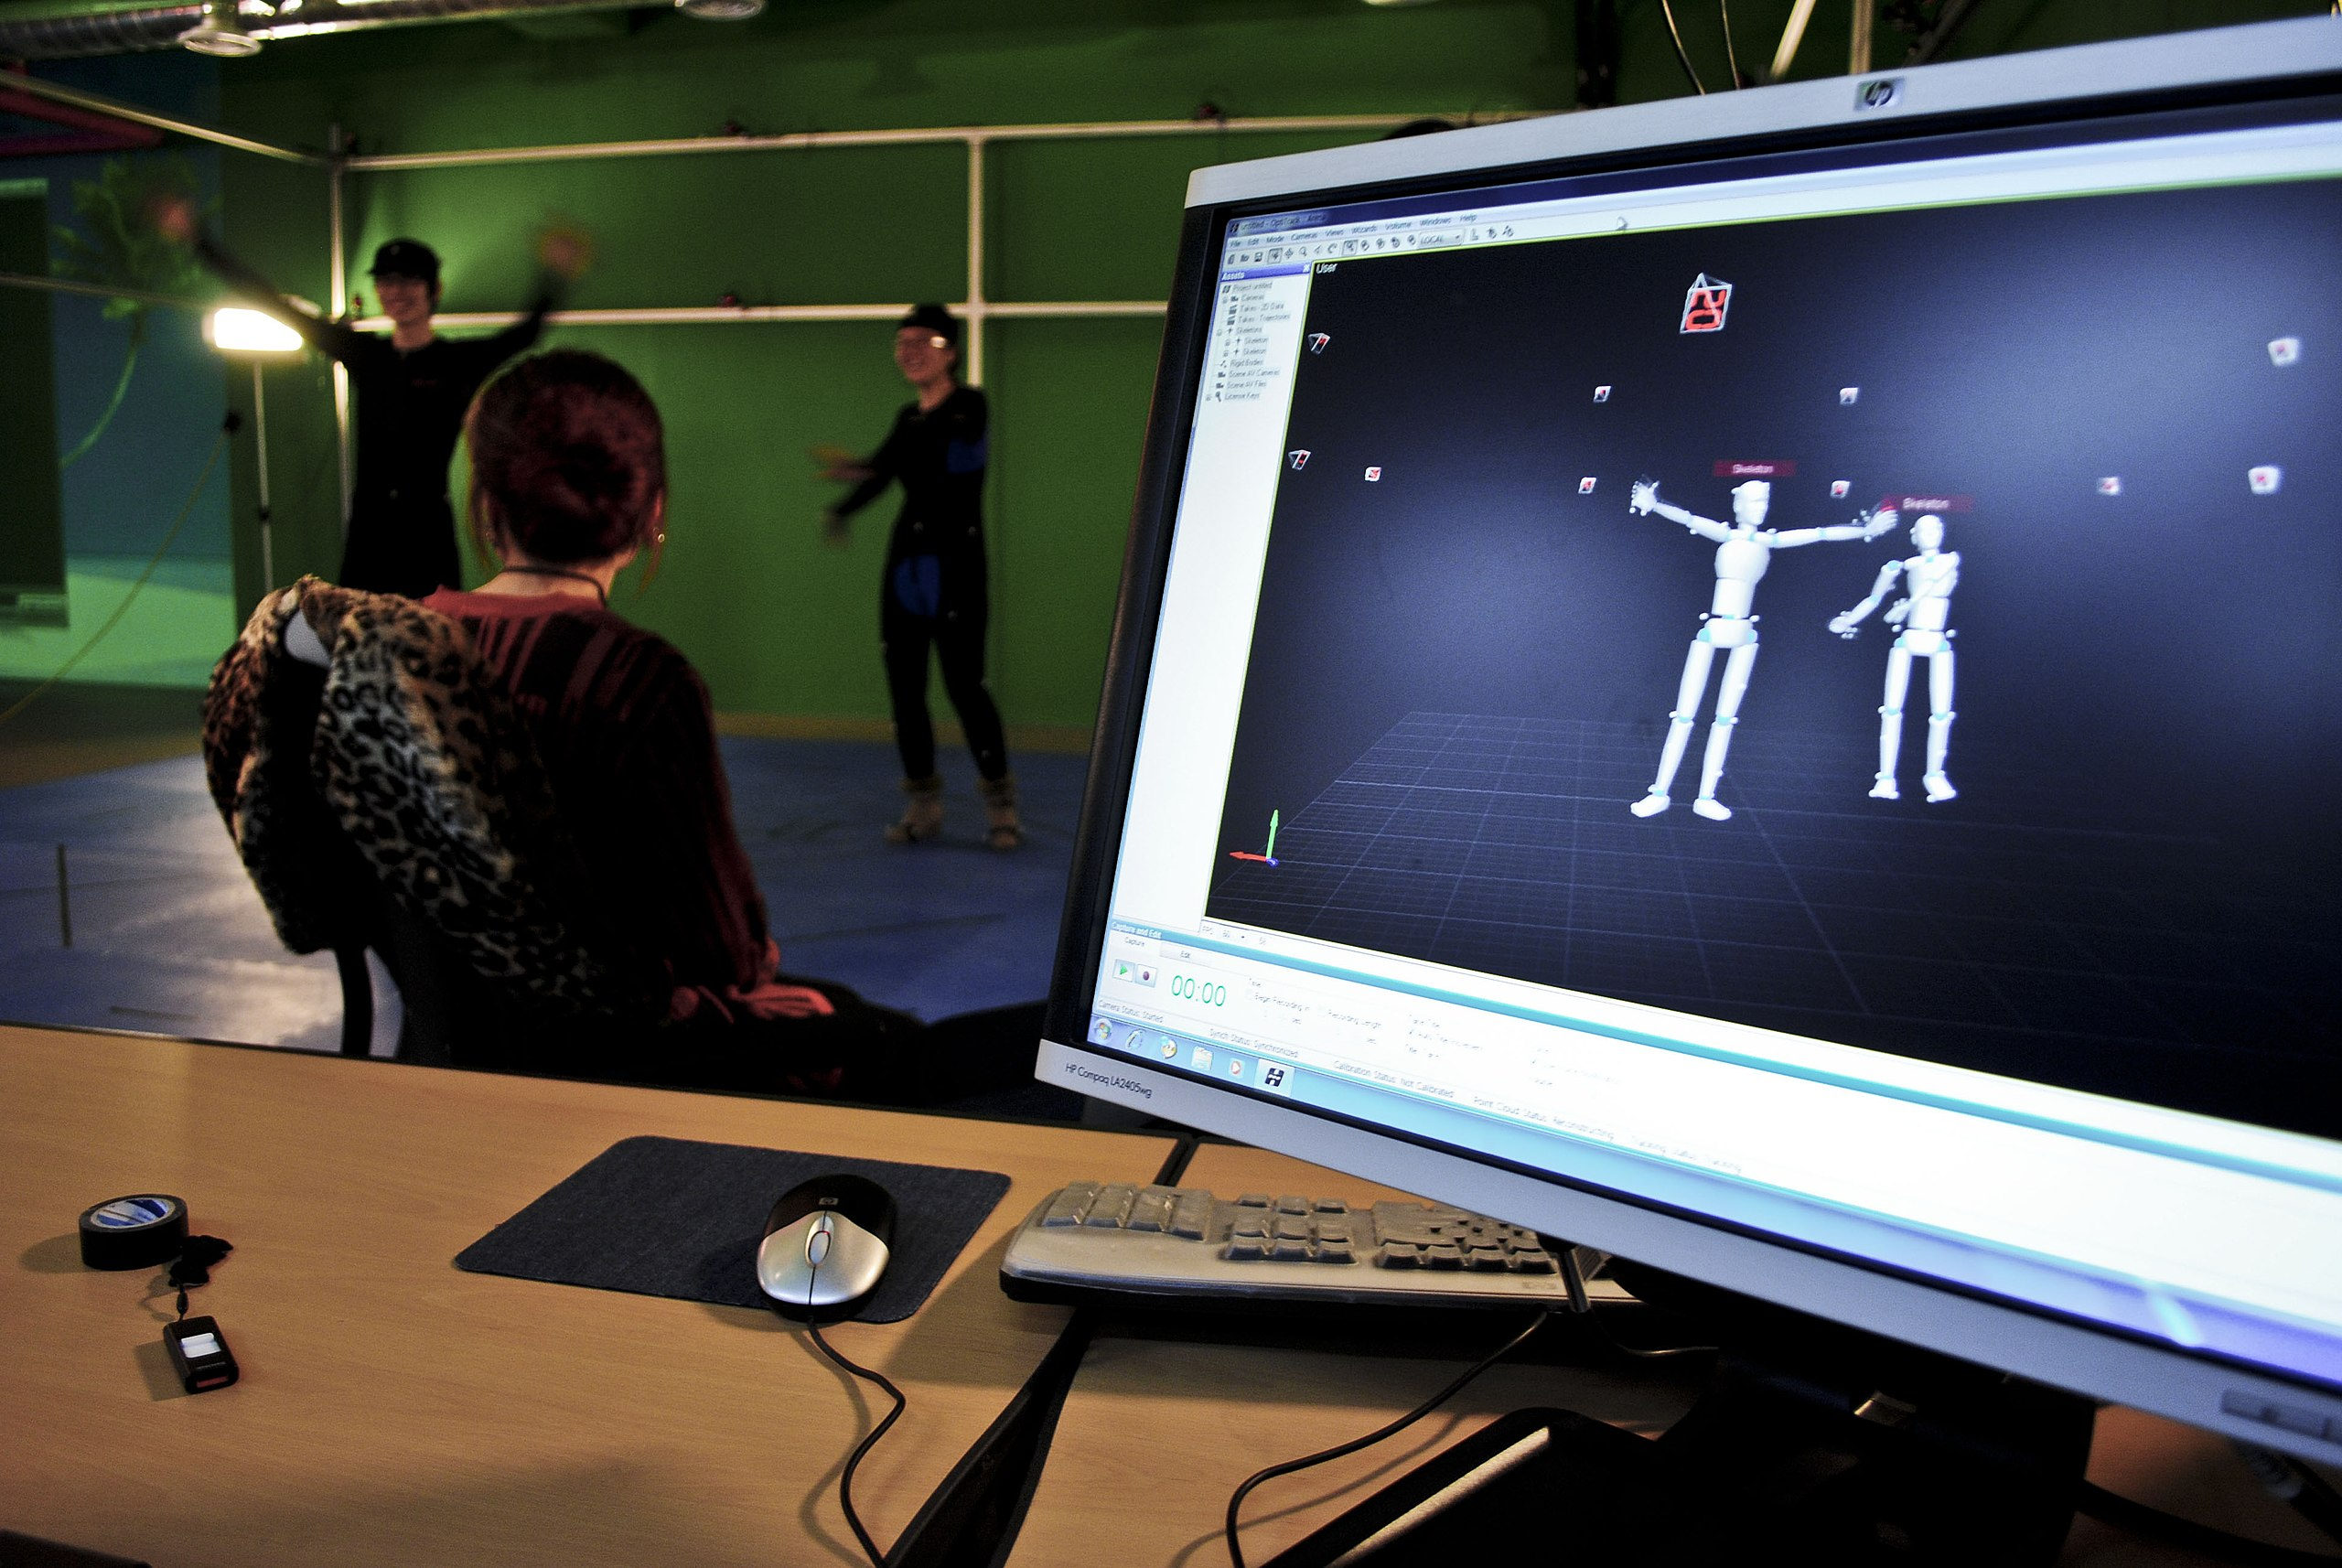
\includegraphics[width = 2.5in]{chapters/background_work/images/mocap.png} 
  \caption{Mocap capture and retargeting} 
  \label{fig:mocap} 
\end{figure}

Motion capture (mocap) retargeting offers a significant boost in animation speed and realism, but it does come with its challenges. It requires specialized equipment and involves intricate data processing, particularly when filtering out noise. Additionally, reusing mocap data across different avatars can be complex due to variations in body proportions and joint placements. Furthermore, segmenting mocap data into different parts for reuse can be difficult, limiting its flexibility in animation projects.

\paragraph{Kinematics}
\label{ch:background_work:sign_language_synthesis:3d_techniques:avatar_animation:kinematics}

Kinematics is used to define the motion of joints in a skeleton, allowing animators to create realistic and dynamic movements. Two key kinematic techniques used in avatar animation are forward kinematics (FK) and inverse kinematics (IK).

\subparagraph{Forward Kinematics}
\label{ch:background_work:sign_language_synthesis:3d_techniques:avatar_animation:kinematics:forward_kinematics}

Forward kinematics (FK) is a method where the position and rotation of each joint in a skeleton are specified explicitly by the animator. This means that to move a hand, for example, the animator must adjust the shoulder, elbow, and wrist joints individually. FK provides precise control over each joint, making it ideal for detailed and deliberate animations. However, it can be cumbersome for complex movements, as changes to one joint may require adjustments to multiple other joints to achieve a natural pose. Figure~\ref{fig:forward_kinematics_example} illustrates the forward kinematics process.

\begin{figure} 
  \centering 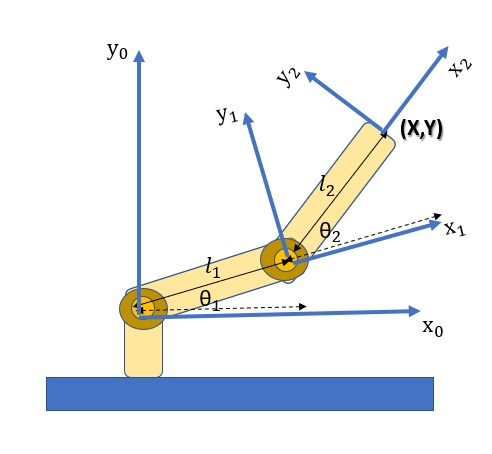
\includegraphics[width = 2.5in]{chapters/background_work/images/forward_kinematics_example.png} 
  \caption{Forward kinematics} 
  \label{fig:forward_kinematics_example} 
\end{figure}

\subparagraph{Inverse Kinematics}
\label{ch:background_work:sign_language_synthesis:3d_techniques:avatar_animation:kinematics:inverse_kinematics}

Inverse kinematics (IK) simplifies the animation process by allowing the animator to position the end effector (e.g., a hand or foot) directly, and the software automatically calculates the necessary joint rotations to achieve this position. This technique is particularly useful for tasks like making a character’s hand reach a specific point or ensuring that feet remain planted on the ground. IK is widely used in character animation to create natural and realistic movements more efficiently than FK.

IK solvers are algorithms that compute the necessary joint rotations to achieve a desired position of the end effector. Different IK solvers are available, each with its unique approach and strengths. Here are a few popular IK solvers:

\begin{itemize} 
  \item \textbf{iTaSc (Instantaneous Task Specification using Constraints)}: iTaSc~\cite{4648032} operates by formulating the IK problem as a set of instantaneous task specifications, which are treated as constraints. These \gls{posture_constraint}s can include positions, orientations, and other task-specific requirements. The method solves the IK problem by minimizing a cost function subject to these constraints. It utilizes optimization techniques to handle multiple, potentially conflicting \gls{posture_constraint}s simultaneously, ensuring that the solution adheres to the defined task requirements.

  \item \textbf{CCDIK (Cyclic Coordinate Descent Inverse Kinematics)}: CCDIK~\cite{kenwright2012inverse} works by iteratively optimizing the position of each joint in the kinematic chain. Starting from the end effector, the algorithm adjusts each joint to minimize the distance between the end effector and the target position. This is done in a cyclic manner, where each joint is adjusted in sequence until the end effector reaches an acceptable proximity to the target. The process is repeated iteratively, ensuring that the adjustments of one joint do not significantly disrupt the adjustments of previous joints.

  \item \textbf{FABRIK (Forward And Backward Reaching Inverse Kinematics)}: FABRIK~\cite{aristidou2011fabrik} operates through a two-phase iterative process: forward reaching and backward reaching. In the forward reaching phase, the algorithm starts from the base of the kinematic chain and moves towards the end effector, adjusting each joint to align with the target position while respecting joint constraints. In the backward reaching phase, the algorithm starts from the end effector and moves back towards the base, further refining joint positions to ensure convergence towards the target. This alternating process continues until the end effector reaches the desired target within an acceptable tolerance.
\end{itemize}

Figure~\ref{fig:inverse_kinematics_example} illustrates the inverse kinematics process.

\begin{figure} 
  \centering 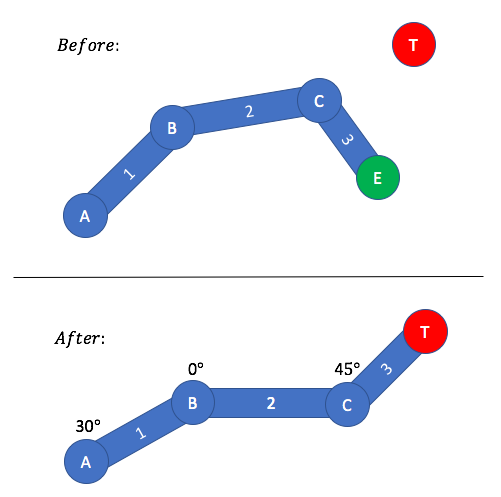
\includegraphics[width = 2.5in]{chapters/background_work/images/inverse_kinematics_example.png} 
  \caption{Inverse kinematics} 
  \label{fig:inverse_kinematics_example} 
\end{figure}


Both multi-track and non-linear editing have been widely used in various fields, including film production, video editing(figure~\ref{fig:video_edit}), and animation (figure~\ref{fig:nle_blender}). 

\begin{figure}[h]
    \centering
    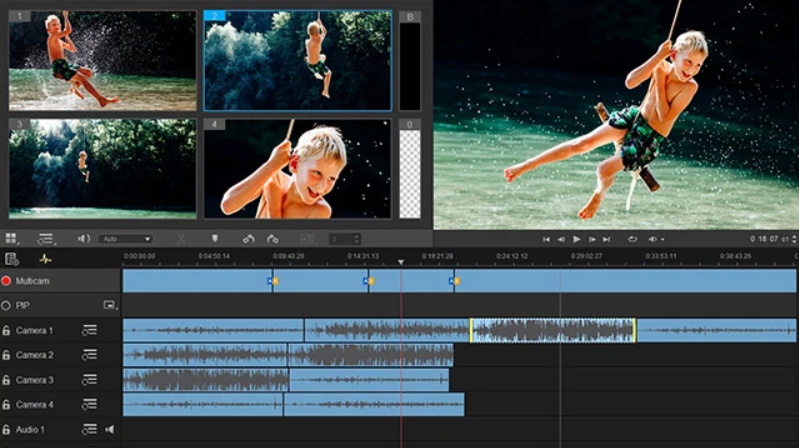
\includegraphics[width=0.8\textwidth]{chapters/multi_track/images/video_editing.png}
    \caption{Video editing software interfaces with multiple tracks for editing video and audio clips.}
    \label{fig:video_edit}
\end{figure}

\begin{figure}[h]
    \centering
    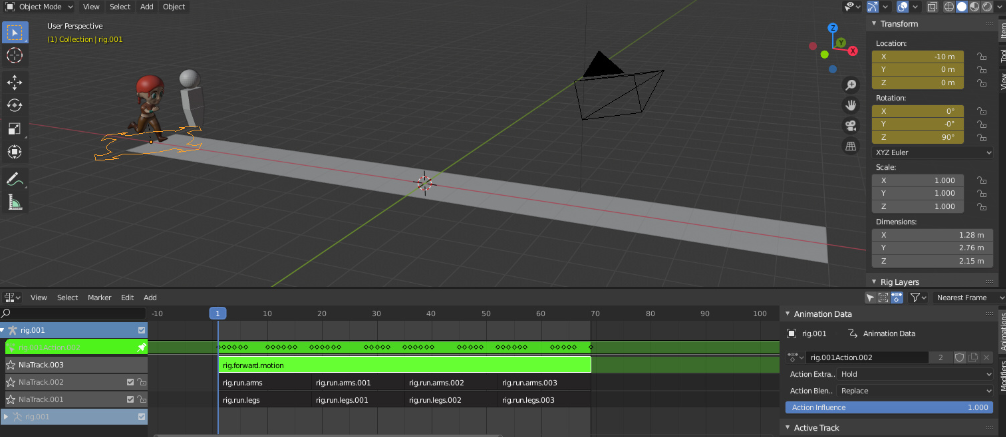
\includegraphics[width=0.8\textwidth]{chapters/multi_track/images/nle_blender.png}
    \caption{Blender's non-linear editor interface showing multiple tracks for editing animation clips.}
    \label{fig:nle_blender}
\end{figure}

\subsection{Existing low-level AZee synthesizor}
\label{ch:multi_track:related_work:old_azee_synthesizor}

Although AZee is multi-track by nature (where the lingusit has the ability to crate the track), the low-level AZee synthesizor is based on a flattened \emph{AnimatedScore} representation that flattenes each track made by the linguist. This flattening layer loses the multi-track information and the dynamics of the original AZee description. 

For example, consider the following low-level AZee description for \emph{:cupboard} when compiled with the AZee interpreter generates an AZee \emph{SyncedScore} using the algorithm~\ref{alg:azee_recursion}~\cite{filhol2017synthesizing} that is show in in figure~\ref{fig:azee_synced_score}.

\begin{figure}[h]
    \centering
    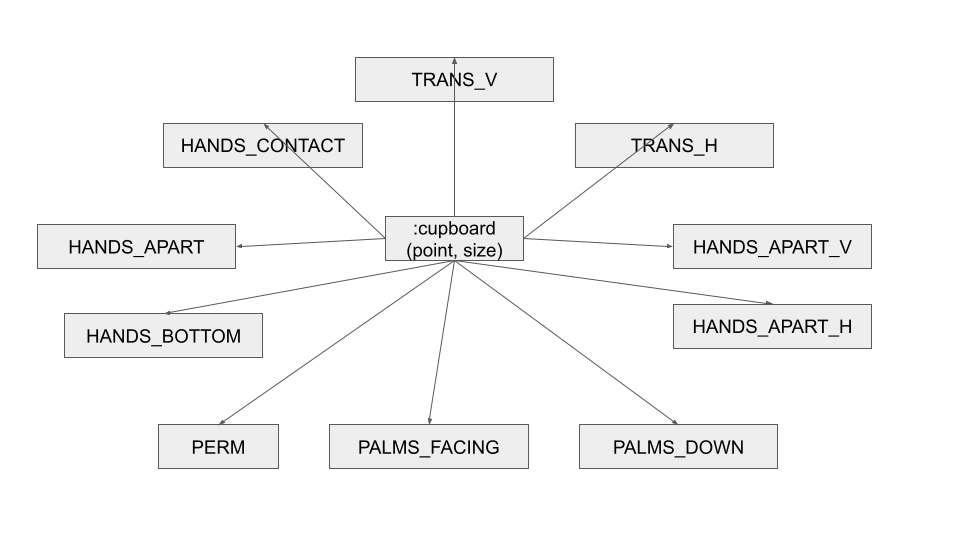
\includegraphics[width=0.8\textwidth]{chapters/multi_track/images/azee_synced_score.png}
    \caption{AZee Synced Score generated from the low-level AZee description.}
    \label{fig:azee_synced_score}
\end{figure}

Figure~\ref{fig:azee_flattened_score} shows the flattened version of this AZee Synced Score, where all the tracks are merged into a single track. This flattening is done by collecting all the \gls{posture_constraint}s for each frame and applying them to the corresponding bone rotations during animation.

\begin{figure}[h]
    \centering
    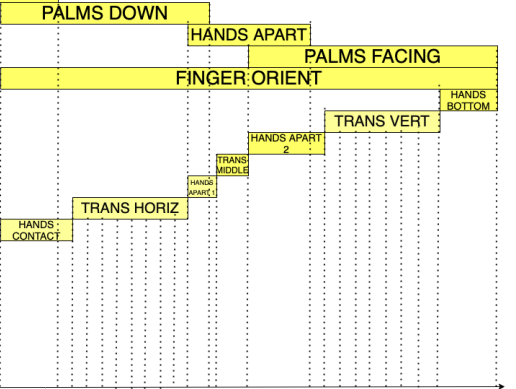
\includegraphics[width=0.8\textwidth]{chapters/multi_track/images/azee_flattened_score.png}
    \caption{Flattened version of the AZee Synced Score.}
    \label{fig:azee_flattened_score}
\end{figure}

This approach is also inextensible to be used with pre-animated motion data blocks for larger sequences since the flattened representation does not contain the original location of the corresponding animation block on the timeline. 

\subsection{Paula}
\label{ch:multi_track:related_work:paula}

On the contrary, a multi-track approach to \gls{sl} synthesis has already been done by~\cite{filhol2017synthesizing}. Paula is a multi-track \gls{sl} synthesis system that strictly uses pre-recorded motion data. The system is based on a multi-track timeline where each track is created by the artist(or can be based on the AZee description). The Paula interface is shown in figure~\ref{fig:paula}.

\begin{figure}[h]
    \centering
    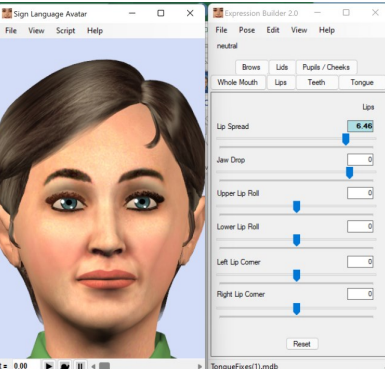
\includegraphics[width=0.8\textwidth]{chapters/multi_track/images/paula.png}
    \caption{Paula interface showing a multi-track timeline for \gls{sl} synthesis.}
    \label{fig:paula}
\end{figure}

However, Paula doesn't support low-level synthesis from AZee descriptions. This poses a challenge in scalability since an artist is always needed to create the building blocks of the animation. Although, the interface is tailored specifically for creating \gls{sl} content, a human intervention is still needed. Another drawback of Paula is that it is based on a single avatar model, which limits the diversity of the animations that can be created.

\subsection{Outside \gls{sl} Synthesis}
\label{ch:multi_track:related_work:other_multi_track}

The concept of multi-track timeline control for text-driven 3D human motion generation was also explored by~\cite{petrovich24stmc}. The work introduces a novel way to address the limitations of previous methods that lacked fine-grained control over action composition and timing. This approach allows users to define multiple textual prompts within overlapping temporal intervals, enabling precise control over complex actions (figure~\ref{fig:multi_track_other}). The proposed Spatio-Temporal Motion Collage (STMC) method, which operates at test-time, integrates with pre-trained motion diffusion models to generate realistic motions that adhere to the specified timeline. However, it is not for use in \gls{sl} synthesis, where precise and context-sensitive hand and body gestures are required, as it relies heavily on models not specifically designed for such detailed tasks.

\begin{figure}
    \centering
    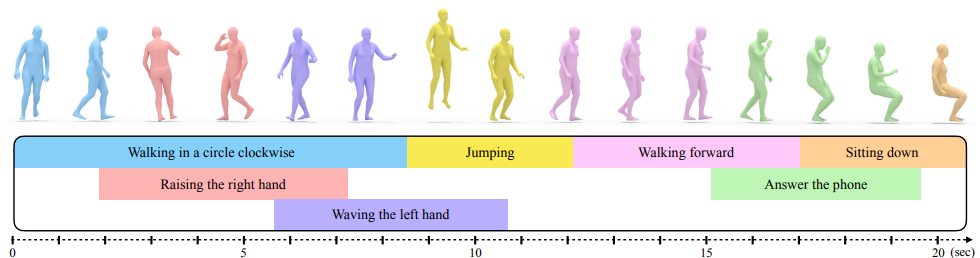
\includegraphics[width=0.8\textwidth]{chapters/multi_track/images/multi_track_other.png}
    \caption{Multi-track timeline control for text-driven 3D human motion generation.}
    \label{fig:multi_track_other}
\end{figure}

 fix this


todo fix pose est 

\section{Related Work}
\label{ch:pose_correction:related_work}

In this section, we discuss the progression of techniques in generating natural poses for character animation, starting from classical IK methods and moving to modern data-driven approaches. We conclude with the use of pose priors in correcting poses for more realistic outcomes, as used in our \gls{sl} animation system.

\subsection{Introduction to Inverse Kinematics (IK)}
\label{ch:pose_correction:related_work:intro_ik}
Inverse Kinematics (IK) is a well-established technique in character animation that computes joint angles to achieve a desired end-effector position. It has found widespread use, but limitations exist, particularly in dynamic and realistic animation contexts.

\subsection{Classical IK Methods and Their Limitations}
\label{ch:pose_correction:related_work:classical_ik}
Classical IK methods, though foundational, face several challenges in handling complex \gls{posture_constraint}s and delivering natural poses in all situations.

\paragraph{Jacobian-Based Methods} Jacobian-based approaches~\cite{4648032} involve calculating the Jacobian matrix to linearize the relationship between joint angles and end-effector positions. By iteratively adjusting joint angles, these methods reduce the error between the current and target positions. Despite their robustness in real-time applications, they suffer from singularities, where solutions become unstable or unrealistic. An example is illustrated in Figure~\ref{fig:jacobian_based}.

\begin{figure}
    \centering 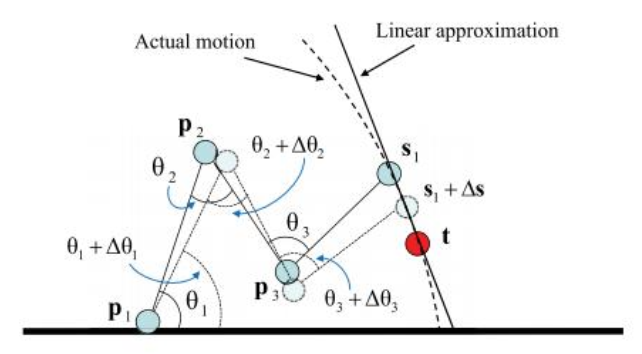
\includegraphics[width = 2.5in]{chapters/pose_correction/images/jacobian_based.png}
    \caption{Jacobian based IK solving (approximation of the first derivative)}
    \label{fig:jacobian_based}
\end{figure}

\paragraph{Cyclic Coordinate Descent (CCD)} CCD~\cite{kenwright2012inverse} simplifies the IK problem by adjusting one joint at a time, minimizing the distance between the end-effector and the target. CCD is computationally efficient and easy to implement, which makes it popular in game engines. However, its greedy approach can lead to suboptimal solutions in more constrained or biomechanically complex setups, as shown in Figure~\ref{fig:ccdik}.

\begin{figure}
  \centering 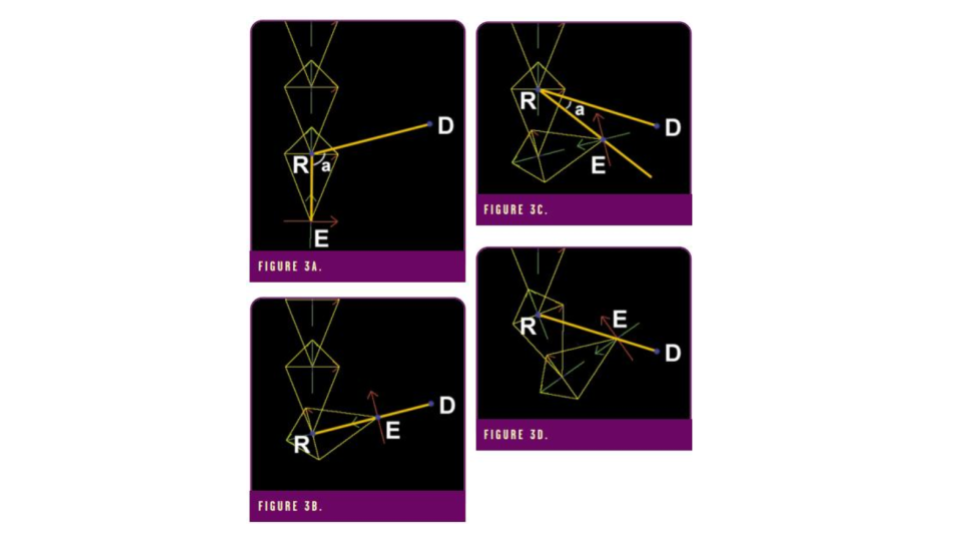
\includegraphics[width = 2.5in]{chapters/pose_correction/images/ccdik.png}
  \caption{Cyclic Coordinate Descent (CCD) IK solving (changes the rotation of a joint, one at a time)}
  \label{fig:ccdik}
\end{figure}

\paragraph{Forward And Backward Reaching Inverse Kinematics (FABRIK)} FABRIK~\cite{aristidou2011fabrik} diverges from other methods by focusing on joint positions rather than angles. It works by iteratively adjusting joint positions in two passes—first from the end-effector to the root, and then from the root to the end-effector. FABRIK is known for its stability and simplicity, particularly in scenarios requiring natural joint configurations, as depicted in Figure~\ref{fig:fabrik}.

\begin{figure}
  \centering 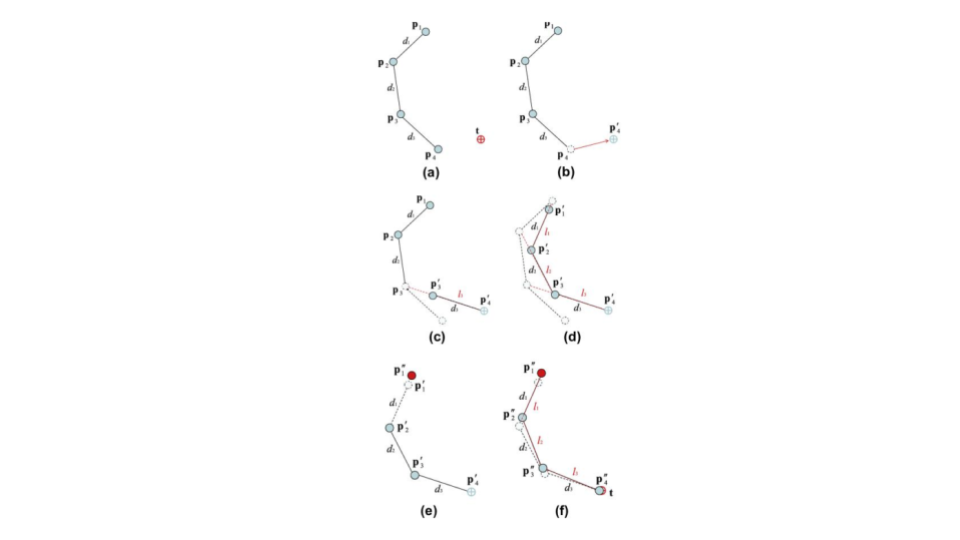
\includegraphics[width = 2.5in]{chapters/pose_correction/images/fabrik.png}
  \caption{Forward And Backward Reaching Inverse Kinematics (FABRIK) solving (updates coordinates in two passes)}
  \label{fig:fabrik}
\end{figure}

\paragraph{Limitations of Classical Methods} These classical IK techniques, while computationally efficient, are prone to singularities, have limited support for complex joint constraints, and often result in unnatural or biomechanically unrealistic poses. As demonstrated in Figure~\ref{fig:problems_classical}, they struggle with overlapping chains and handling multiple end-effectors.

\begin{figure}
  \centering 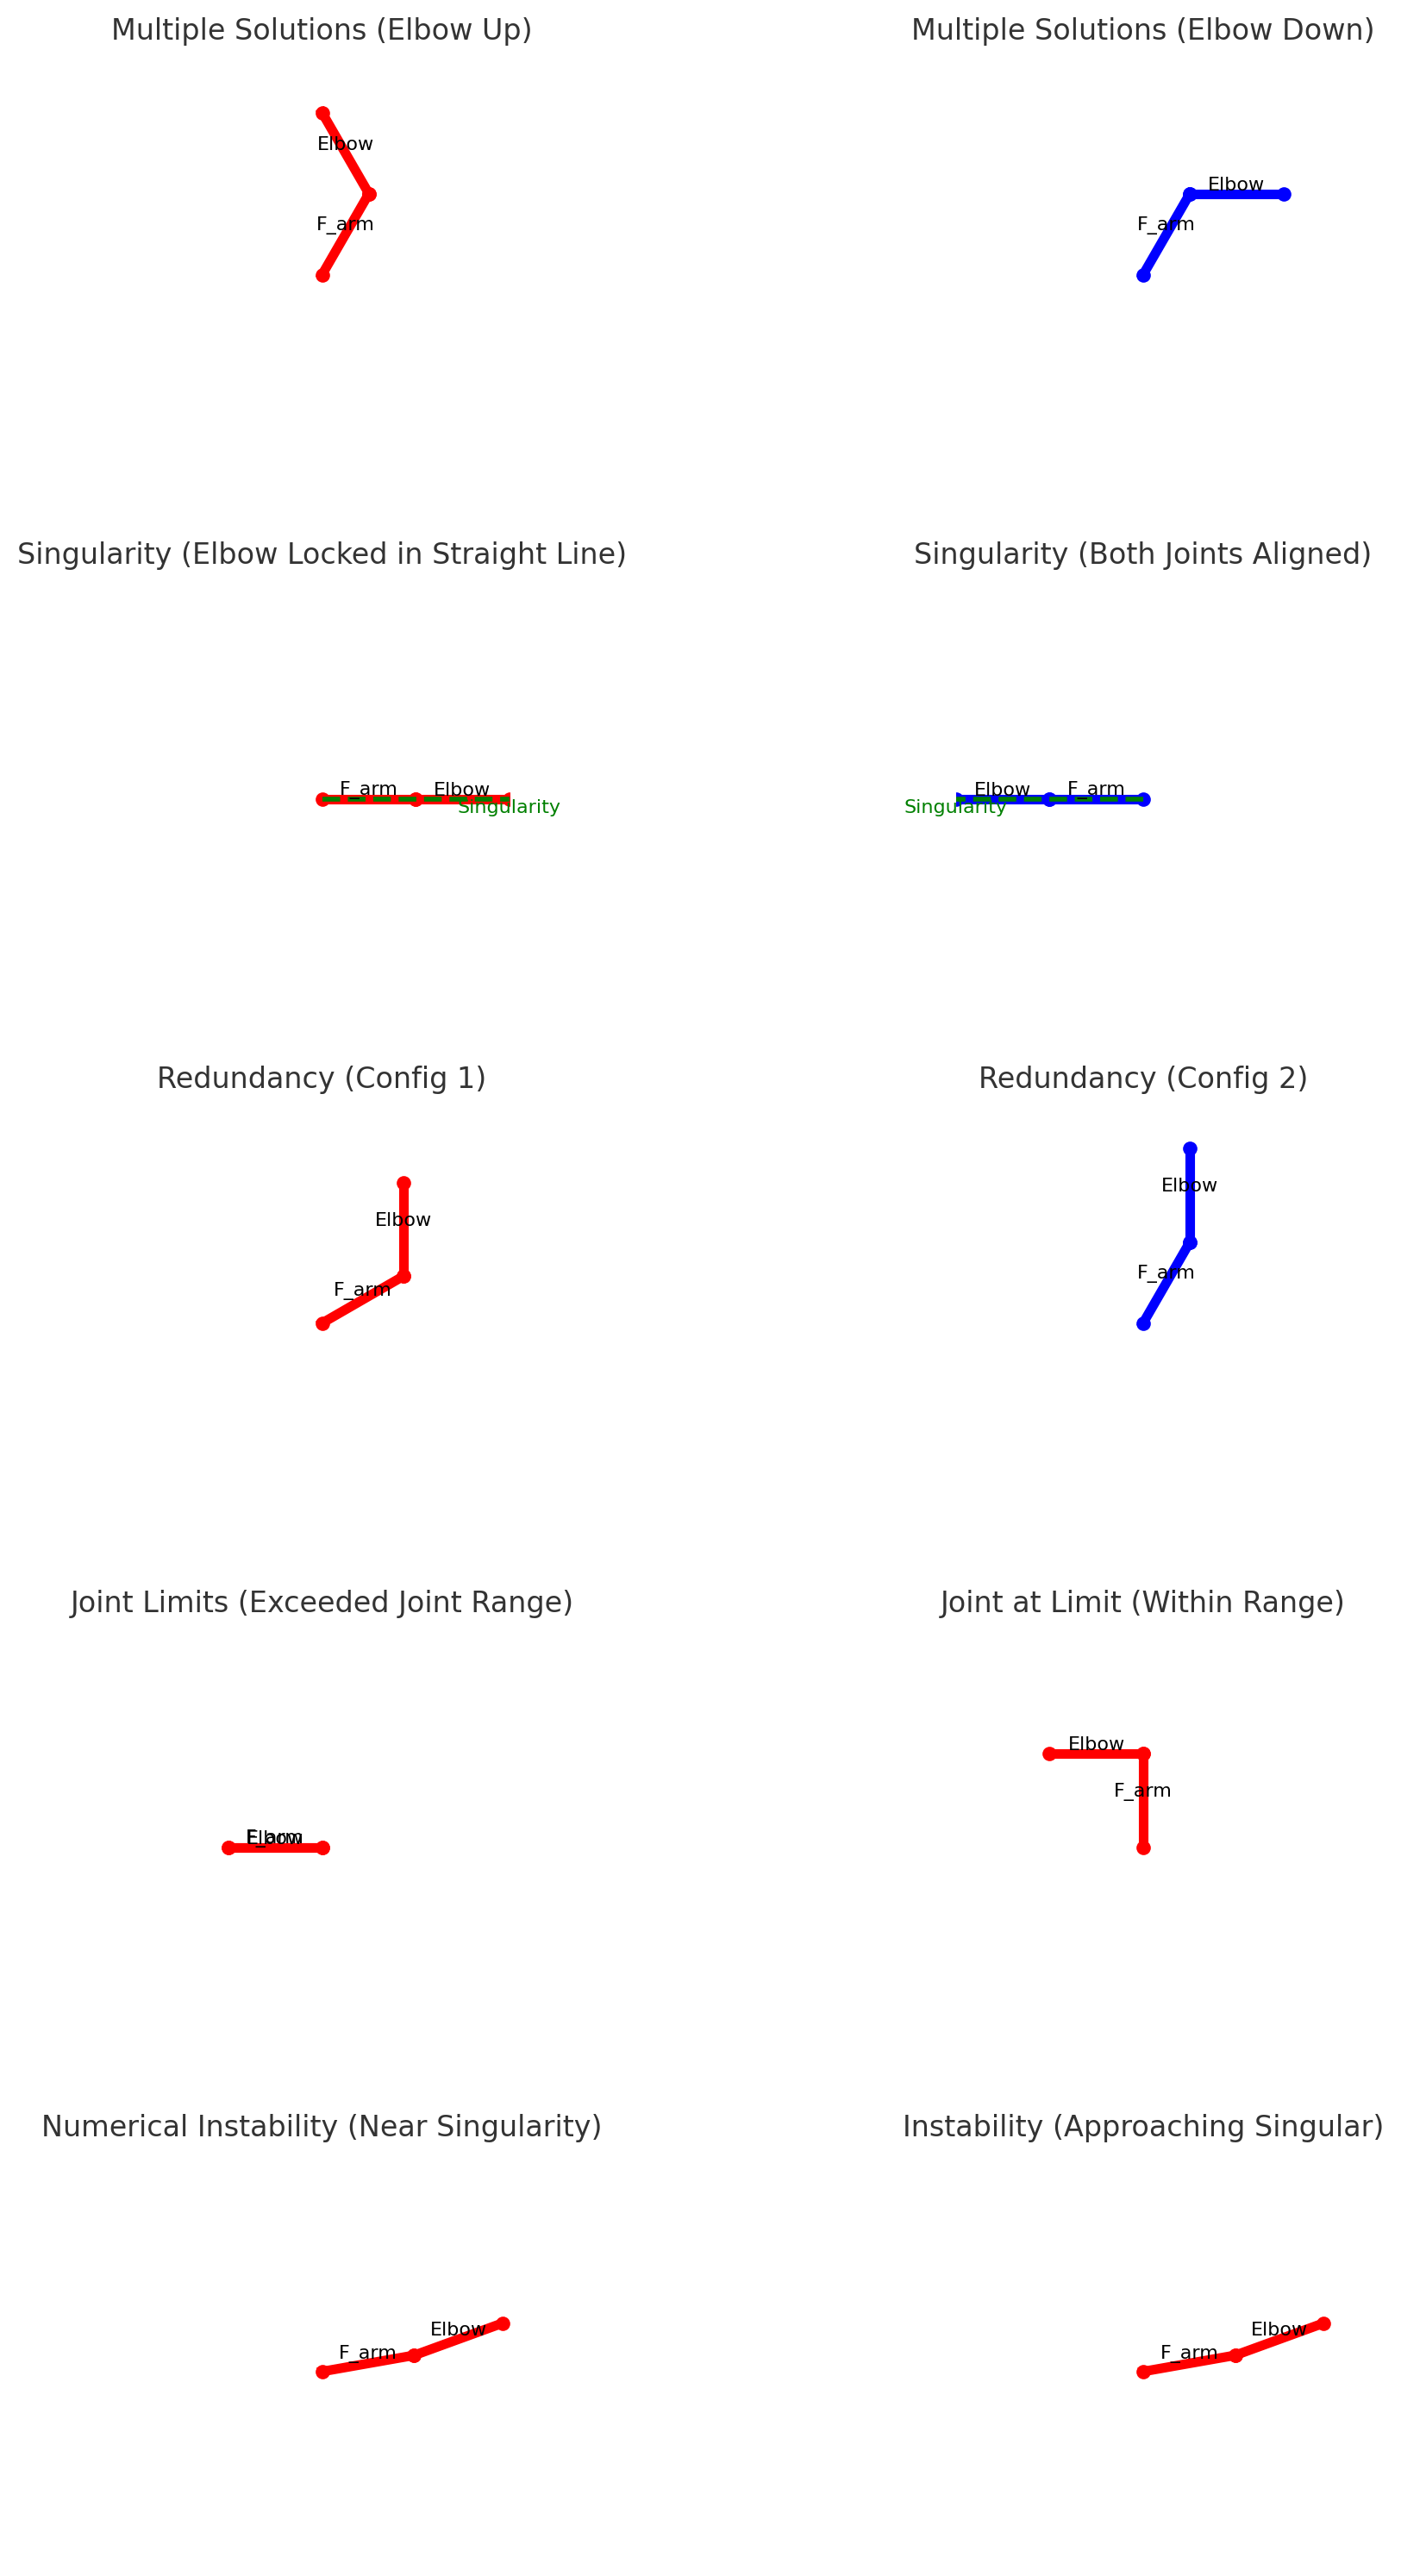
\includegraphics[width = 5in]{chapters/pose_correction/images/problems_classical.png}
  \caption{Problems with classical IK methods}
  \label{fig:problems_classical}
\end{figure}

\subsection{Improved Data-Driven IK Approaches}
\label{ch:pose_correction:related_work:data_driven_ik}
To address the shortcomings of classical IK methods, data-driven approaches have emerged, leveraging large datasets and machine learning to produce more flexible and realistic animations.

\paragraph{Motion Matching} Motion Matching represents a significant shift from traditional techniques by dynamically selecting the most appropriate pose from a large database of motion capture (mocap) data based on user inputs and contextual parameters. Ubisoft's \emph{For Honor} utilized this technique to create more fluid and responsive character animations, as shown in Figure~\ref{fig:for_honor}. Motion Matching's ability to break down animations into fine-grained clips allows for seamless transitions and natural movements.

\begin{figure}
  \centering 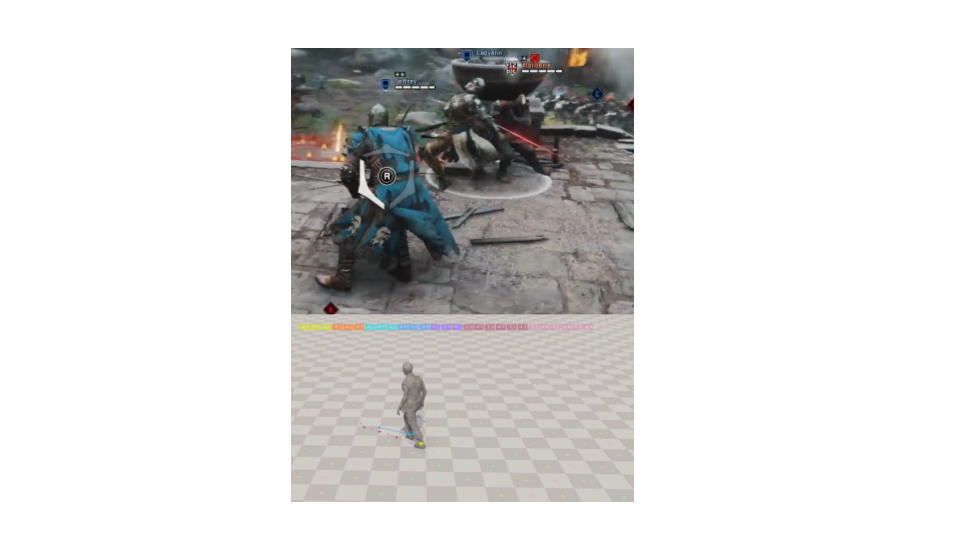
\includegraphics[width = 2.5in]{chapters/pose_correction/images/for_honor.png}
  \caption{Motion Matching in Ubisoft’s \emph{For Honor}}
  \label{fig:for_honor}
\end{figure}

\paragraph{Phase-Functioned Neural Networks (PFNN)} PFNN~\cite{10.1145/3072959.3073663} extends the principles of motion matching by incorporating phase information into the neural network’s weights, allowing the network to generate animations that align with the cyclical nature of bipedal movement (walking, running). Unlike traditional methods that blend animation clips, PFNN encodes the entire animation process within the neural network, providing more control and flexibility, as illustrated in Figure~\ref{fig:pfnn}.

\begin{figure}
  \centering 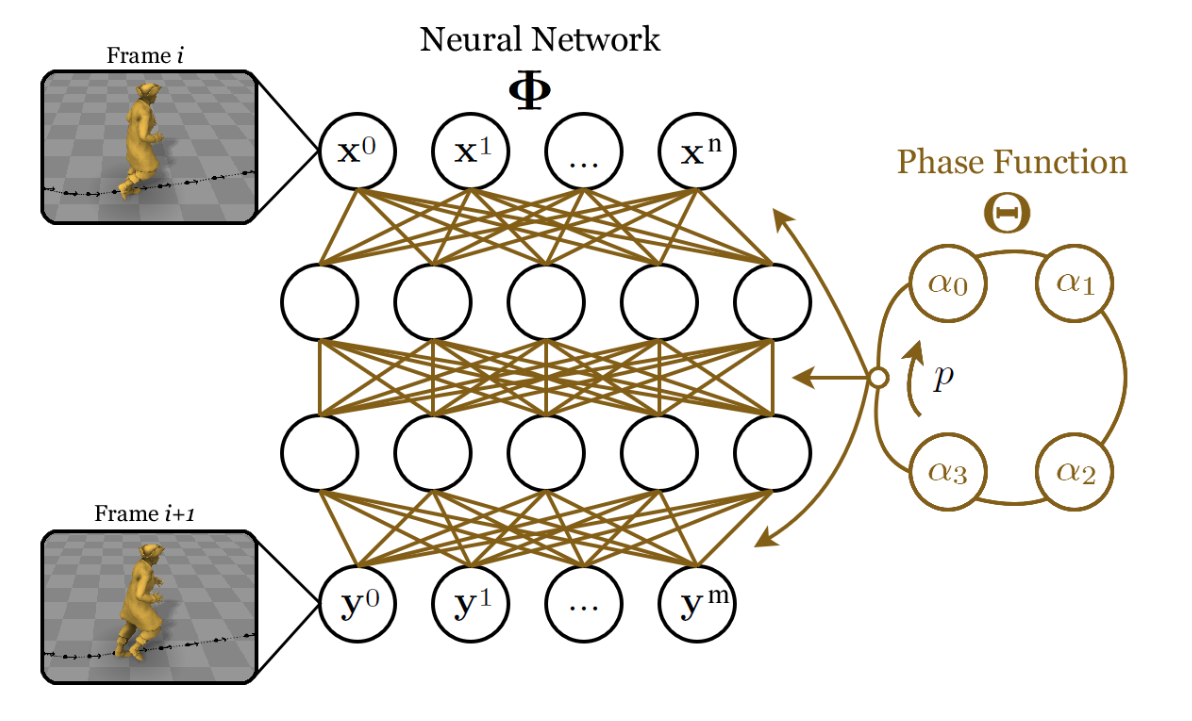
\includegraphics[width = 2.5in]{chapters/pose_correction/images/pfnn.png}
  \caption{Phase-Functioned Neural Networks (PFNN) for motion matching}
  \label{fig:pfnn}
\end{figure}

\paragraph{Style-Based Inverse Kinematics (Style IK)} Style IK~\cite{grochow2004style} leverages machine learning to represent poses in a latent space using Scaled Gaussian Process Latent Variable Models (SGPLVM). By learning the distribution of poses, Style IK generates stylized animations that adhere to aesthetic or functional constraints, making it especially useful in scenarios where mocap data is unavailable or infeasible. Figure~\ref{fig:style_ik} shows how poses are mapped in latent space for Style IK.

\begin{figure}
  \centering 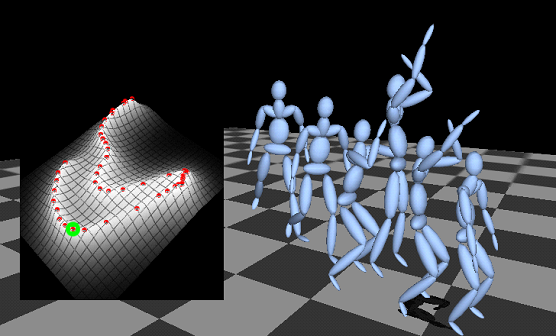
\includegraphics[width = 2.5in]{chapters/pose_correction/images/style_ik.png}
  \caption{Pose in latent space using Style IK}
  \label{fig:style_ik}
\end{figure}

While these data-driven methods resolve many issues inherent to classical IK, they bring challenges like the need for large amounts of training data and increased computational demands, particularly in real-time applications.

\subsection{Latent Space Representations for Pose Generation}
\label{ch:pose_correction:related_work:latent_space}
Latent space representations have become crucial in reducing the complexity of pose and motion data, allowing for more efficient and realistic pose generation and manipulation.

\paragraph{Variational Autoencoders (VAEs) and SMPLify-X} VAEs~\cite{kingma2013auto}, such as those used in SMPLify-X~\cite{pavlakos2019expressive}, learn a probabilistic model of human poses. They can generate and manipulate poses in a lower-dimensional latent space, which can then be sampled to meet specific \gls{posture_constraint}s such as end-effector positions. SMPLify-X is particularly effective in estimating 3D poses from 2D images, as illustrated in Figure~\ref{fig:simplifyx}.

\begin{figure}
  \centering 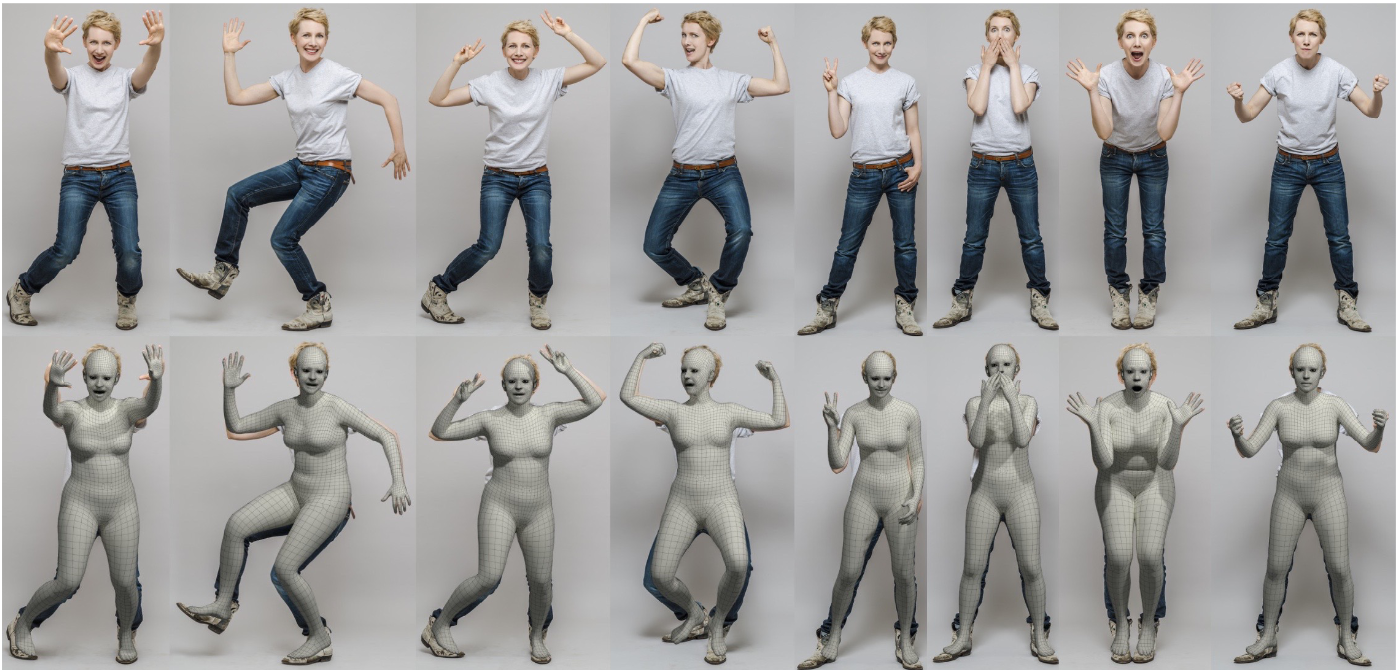
\includegraphics[width = 2.5in]{chapters/pose_correction/images/simplifyx.png}
  \caption{SMPLify-X generating poses from latent space}
  \label{fig:simplifyx}
\end{figure}

\paragraph{VPoser for Pose Correction} VPoser~\cite{pavlakos2019expressive}, a specific implementation of a VAE, encodes human poses into a low-dimensional latent space. This latent space helps regularize pose generation, ensuring that generated poses are realistic and meet specific biomechanical criteria. VPoser plays a critical role in optimization processes by constraining pose generation to physically plausible configurations, as seen in Figure~\ref{fig:vposer}.

\begin{figure}
  \centering \includegraphics[width = 2.5in]{chapters/pose_correction/images/vposer.png}
  \caption{Pose regularization using VPoser in a latent space}
  \label{fig:vposer}
\end{figure}

\subsection{Pose Priors and Corrective Methods}
\label{ch:pose_correction:related_work:pose_priors}
Pose priors provide a mechanism to generate plausible poses based on learned distributions from large datasets. These pose priors ensure that the generated poses are not only valid but also contextually appropriate.

\paragraph{VPoser for Pose Correction in \gls{sl} Animation} In our system, we utilize VPoser to correct the poses generated by the \gls{sl} animation system. By training VPoser on a comprehensive dataset of human poses, we can snap the initial pose to the closest valid pose in the latent space, thereby ensuring realism and accuracy in \gls{sl} gestures. This method ensures that the final poses are biomechanically correct and visually appropriate.

\subsection{Conclusion}
\label{ch:pose_correction:related_work:conclusion}
This review has traced the development of IK techniques, from classical methods to data-driven approaches that leverage latent spaces. The incorporation of pose priors, particularly through VPoser, offers a robust solution for pose correction in our \gls{sl} animation system, allowing for natural and contextually appropriate movements.


todo fix pose est

\paragraph{Procedural Techniques}
\label{ch:background_work:sign_language_synthesis:3d_techniques:avatar_animation:procedural_techniques}

Procedural animation techniques use algorithms and rules to generate motion automatically, rather than relying on manual keyframing or motion capture data. These techniques are particularly useful for creating dynamic and responsive animations that adapt to changing conditions or user interactions. Procedural animation can be applied to various aspects of avatar animation, including locomotion, facial expressions, and secondary motion.

\subparagraph{Data-Driven Constraint-Based Motion Editing}
\label{ch:background_work:sign_language_synthesis:3d_techniques:avatar_animation:procedural_techniques:data_driven_constraint_based_motion_editing}

Data-driven constraint-based motion editing~\cite{inbook} combines model-based and goal-directed techniques to enhance human motion animation. The system incorporates Prioritized Inverse Kinematics (PIK) to solve for joint movements that meet user-defined constraints. Animators can use key-frame and key-trajectory \gls{posture_constraint}s to specify end-effector positions and paths, simplifying the animation process. The optimization step ensures smooth, continuous motions, avoiding common artifacts and preserving the natural flow of movement.

\subparagraph{Deep Learning based Techniques}
\label{ch:background_work:sign_language_synthesis:3d_techniques:avatar_animation:procedural_techniques:deep_learning_based_techniques}

Deep learning-based techniques have shown significant promise in procedural animation, particularly in the generation of realistic and dynamic movements. Neural networks can be trained on large datasets of motion data to learn complex patterns and generate new animations. For example, diffusion models have been used to synthesize human-like motion sequences with high fidelity and diversity from text prompts. Treating character animation as a cross-modal translation task where descriptive sentences serve as inputs to generate corresponding avatar animations. These techniques, however, require large amounts of data and computational resources to train effectively. Figure~\ref{fig:deep_learning_synthesis} shows an example of deep learning-based synthesis.

\begin{figure} 
  \centering 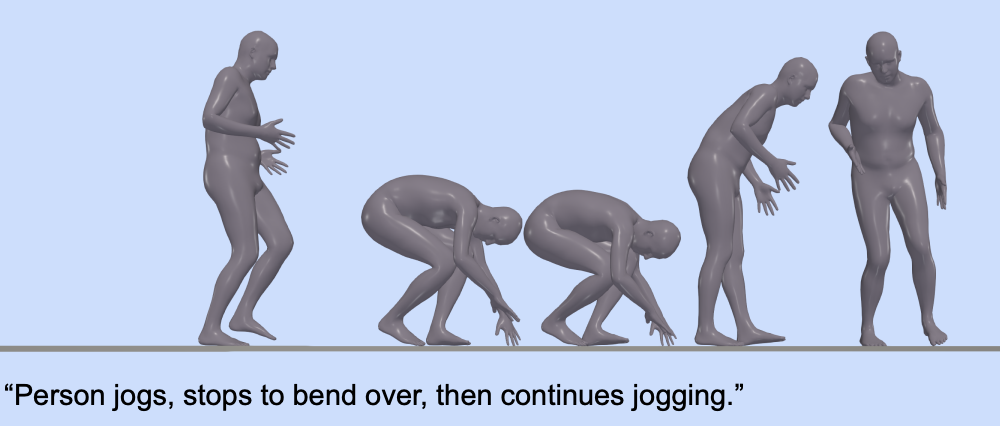
\includegraphics[width = 2.5in]{chapters/background_work/images/deep_learning_synthesis.png} 
  \caption{Deep Learning based synthesis} 
  \label{fig:deep_learning_synthesis} 
\end{figure}

\paragraph{Hybrid Workflows}
\label{ch:background_work:sign_language_synthesis:3d_techniques:avatar_animation:hybrid_workflows}

Hybrid worflows combine elements of manual keyframing, mocap retargeting, and procedural techniques to leverage the strengths of each method. By integrating these approaches, animators can achieve a balance between control, efficiency, and realism. For instance, an animator might use mocap data as a base and then refine specific movements with manual keyframes to enhance expressiveness. Additionally, procedural techniques can be applied to automate repetitive tasks or to ensure that certain \gls{posture_constraint}s are met dynamically during the animation process. Hybrid methods offer a flexible and powerful workflow, allowing for the creation of complex animations that are both realistic and tailored to the specific needs of a project. Figure~\ref{fig:cascadeur} shows an example of a hybrid animation tool, Cascadeur.

\begin{figure} 
  \centering 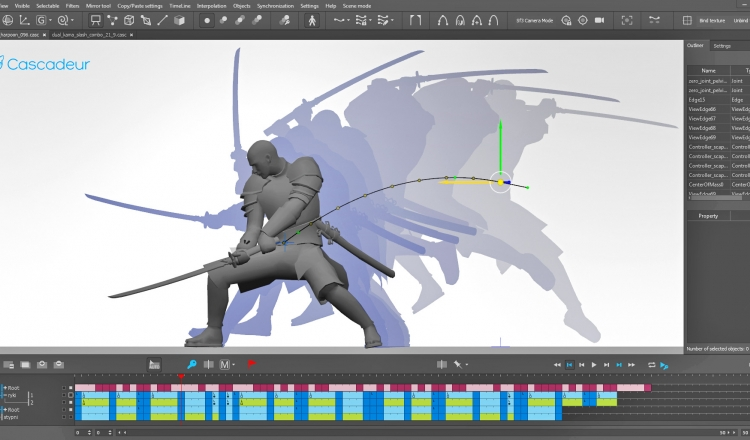
\includegraphics[width = 2.5in]{chapters/background_work/images/cascadeur.png} 
  \caption{Cascadeur hybrid animation tool} 
  \label{fig:cascadeur} 
\end{figure}

todo fix face ex

\section{Related Work}
\label{ch:facial_expressions:related_work}

This section reviews the previous work in facial expression synthesis, focusing on the challenges and advancements in capturing the nuances of facial movements. It also discusses the importance of facial expressions in \gls{sl} synthesis and the techniques used to model these expressions effectively.

\subsubsection{Facial Expressions Synthesis}
\label{ch:facial_expressions:related_work:facial_expressions_synthesis}

Most of the facial expressions research is motivated by synthesis from voice signals. These methods are generally categorized into lip-sync techniques~\cite{yousaidthat, talkingface, lipmovements, lipsyncexpert}, which align mouth movements with audio, and full-face expression synthesis~\cite{eskimez, greenwood18, controllable_facial_synth}. Some approaches model speaking style with 3D animation parameters~\cite{cudeiro}, create generalized latent audio expressions combined with a person-specific 3D model~\cite{FLAME}, and produce expressive facial outputs conditioned on style, although some are unsuitable for tasks requiring full-face movement~\cite{imitating}. A related work, MakeItTalk~\cite{Yang:2020:MakeItTalk}, introduces a two-stage deep learning model that predicts facial landmark displacements based on audio input and a speaker identifier, followed by an image-to-image translation method to generate the final facial expression. Another study, EAMM~\cite{eamm}, focuses on transferring local emotional deformations to an audio-driven talking face, using deep learning to map audio to keypoints and their dynamics, resulting in emotion-related facial motions.

Synthesis of facial expressions in \gls{sl} is a much-less explored area. SGNify~\cite{Forte_2023_CVPR} can do a 3D reconstruction of a signer's face using in FLAME~\cite{FLAME} space from a monocular video. The Paula avatar uses rotational pivots and pre-defined movements, offering more natural and expressive facial animations~\cite{johnson-2022-improved}. More recent work~\cite{azevedo2024empowering} uses sentiment and semantic information to generate realistic facial expressions, achieving state-of-the-art results and outperforming existing approaches. However, these methods are limited in their ability to capture the full range of facial expressions in sign language, particularly the grammatical and emotional nuances that are essential for effective communication. However, these methods are limited in their ability to meaningully relate facial expressions to the signed message.

\subsection{Emotion Recognition}
\label{ch:facial_expressions:related_work:emotion_recognition}

Emotion recognition systems typically use machine learning algorithms to analyze facial features and identify the underlying emotional state. These systems can be trained on large datasets of facial images, which are annotated with emotional labels, to learn the relationships between facial movements and emotions. The most common approach to define emotions is the Ekman's Facial Action Coding System (FACS)~\cite{ekman1978facial}, which categorizes facial expressions into a set of action units (AUs) (figure~\ref{ch:facial_expressions:fig:action_units})  that correspond to specific muscle movements. Recent works by~\cite{luo2022learning} have shown that deep learning models can infer the set of active action units on a face image, which can be used to predict the underlying emotion. EMOCA~\cite{danvevcek2022emoca} is another work which reconstructs 3D faces from single images, accurately capturing emotional expressions by introducing an emotion-consistency loss, significantly improving the quality of reconstructed expressions over previous methods.

\begin{figure}
    \centering
    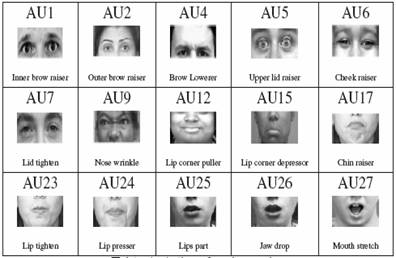
\includegraphics[width=0.8\textwidth]{chapters/facial_expressions/images/action_units.jpg}
    \caption{Facial Action Coding System (FACS) action units}
    \label{ch:facial_expressions:fig:action_units}
\end{figure}

Emotion recognition can be helpful in understanding as well as modeling facial expressions in \gls{sl} synthesis. By analyzing the emotional content of a signed message, we can generate facial expressions that align with the emotional tone of the message, enhancing the realism and expressiveness of the signing avatar.

\subsection{Face Rigging}
\label{ch:facial_expressions:related_work:face_rigging}

Face rigging is the process of creating a digital framework that allows for the animation of facial expressions. There are several approaches to face rigging, each with its advantages and disadvantages. The most common approaches include blendshape-based rigging and skeleton-based rigging.

\subsubsection{Blendshape-Based Rigging}
\label{ch:facial_expressions:related_work:face_rigging:blendshape_based_rigging}

Blendshape-based rigging involves creating a set of predefined facial shapes (blendshapes) that represent various expressions. These blendshapes can be blended together in different proportions to create a wide range of facial expressions. This method is widely used in the animation industry due to its simplicity and flexibility. It allows animators to create complex expressions by adjusting the influence of each blendshape on the final animation. However, the downside of this approach is that it requires a large number of blendshapes to capture all possible expressions, which can be time-consuming to create and manage.

Blendshapes are particularly effective for capturing specific facial movements, such as eyebrow raises, lip curls, cheek puffs, etc. By creating a library of blendshapes that correspond to different facial actions, animators can easily combine these shapes to create expressive and realistic facial animations (figure~\ref{ch:facial_expressions:fig:blendshapes}).

\begin{figure}
    \centering
    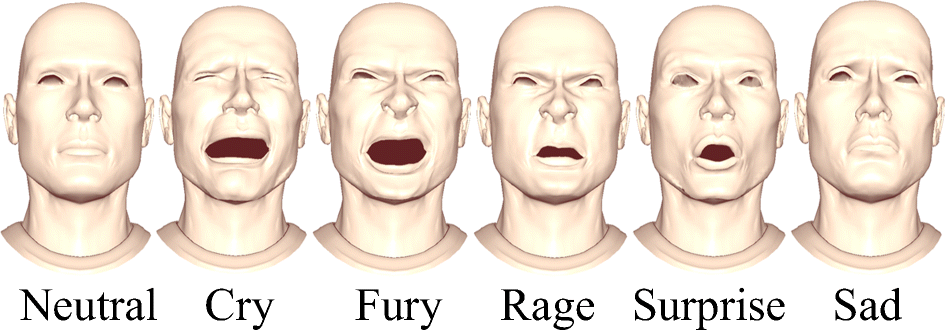
\includegraphics[width=0.8\textwidth]{chapters/facial_expressions/images/blendshapes.png}
    \caption{Blendshapes for facial expressions}
    \label{ch:facial_expressions:fig:blendshapes}
\end{figure}

\subsubsection{Skeleton-Based Rigging}
\label{ch:facial_expressions:related_work:face_rigging:skeleton_based_rigging}

Skeleton-based rigging, also known as joint-based rigging, uses a hierarchical system of bones and joints to control facial movements. This approach is more commonly used for animating body movements but can also be applied to facial animation. The advantage of skeleton-based rigging is that it provides more ways to control since the control space of joints can be 3D (figure~\ref{ch:facial_expressions:fig:skeleton_based_rigging}). Example, jaw movements(up, down, left, right, front or back), eye movements, etc. However, it can be less intuitive to work with compared to blendshapes, especially for subtle expressions that require precise control over individual facial muscles.

%todo better diag
\begin{figure}
    \centering
    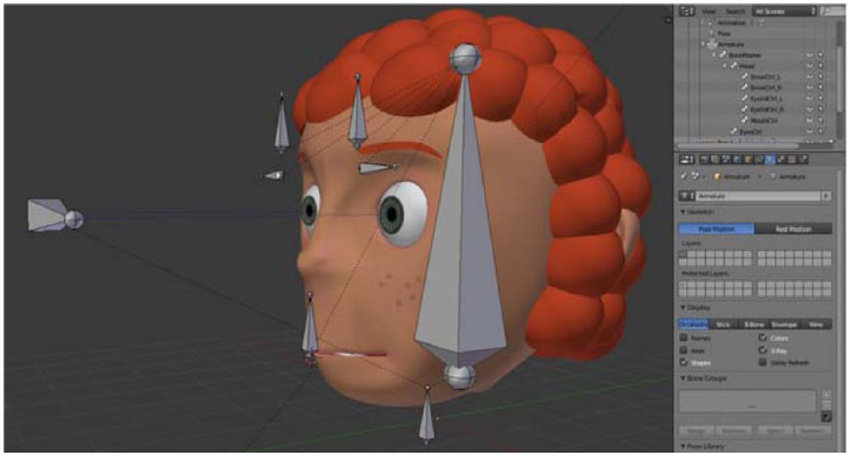
\includegraphics[width=0.8\textwidth]{chapters/facial_expressions/images/skeleton_based_rigging.png}
    \caption{Skeleton-based rigging for facial expressions}
    \label{ch:facial_expressions:fig:skeleton_based_rigging}
\end{figure}

\subsubsection{Hybrid Rigging}
\label{ch:facial_expressions:related_work:face_rigging:hybrid_rigging}

Hybrid rigging approaches combine elements of both blendshape-based and skeleton-based rigging to offer greater flexibility and control. By leveraging the strengths of both techniques, hybrid rigging can overcome the limitations of each individual approach. For example, blendshapes can be used for fine-tuned expressions, while skeletons provide control over broader movements like jaw or head rotations. 

\subsection{Capturing Facial Expressions}
\label{ch:facial_expressions:related_work:face_rigging:capture}

Manual keyframing and performance-based motion capture are some common means to capture facial expressions .

\subsubsection{Manual Keyframing}
\label{ch:facial_expressions:related_work:face_rigging:capture:manual_keyframing}

Keyframing remains a foundational technique in facial animation, where animators manually set key poses and interpolate between them to create fluid motion. While keyframing is effective in controlled environments, it may struggle to capture the natural variability and complexity required in \gls{sl} synthesis, where subtle changes in expression can convey different meanings.

\begin{figure}
    \centering
    \includegraphics[width=0.8\textwidth]{chapters/facial_expressions/images/keyframing.png}
    \caption{Keyframing process, showing how key poses are set and interpolated to create a continuous animation.}
    \label{ch:facial_expressions:fig:keyframing}
\end{figure}

\subsubsection{Performance-Based Motion Capture}
\label{ch:facial_expressions:related_work:face_rigging:capture:performance_based_motion_capture}

Performance-based approaches, such as motion capture, involve capturing real human facial movements and using this data to drive digital avatars. This method provides a high level of realism, capturing the natural dynamics and nuances of facial expressions. Apple's ARKit and FaceCap are examples of performance-based facial animation tools that use motion capture technology to animate digital characters (figure~\ref{ch:facial_expressions:fig:motion_capture}).

\begin{figure}
    \centering
    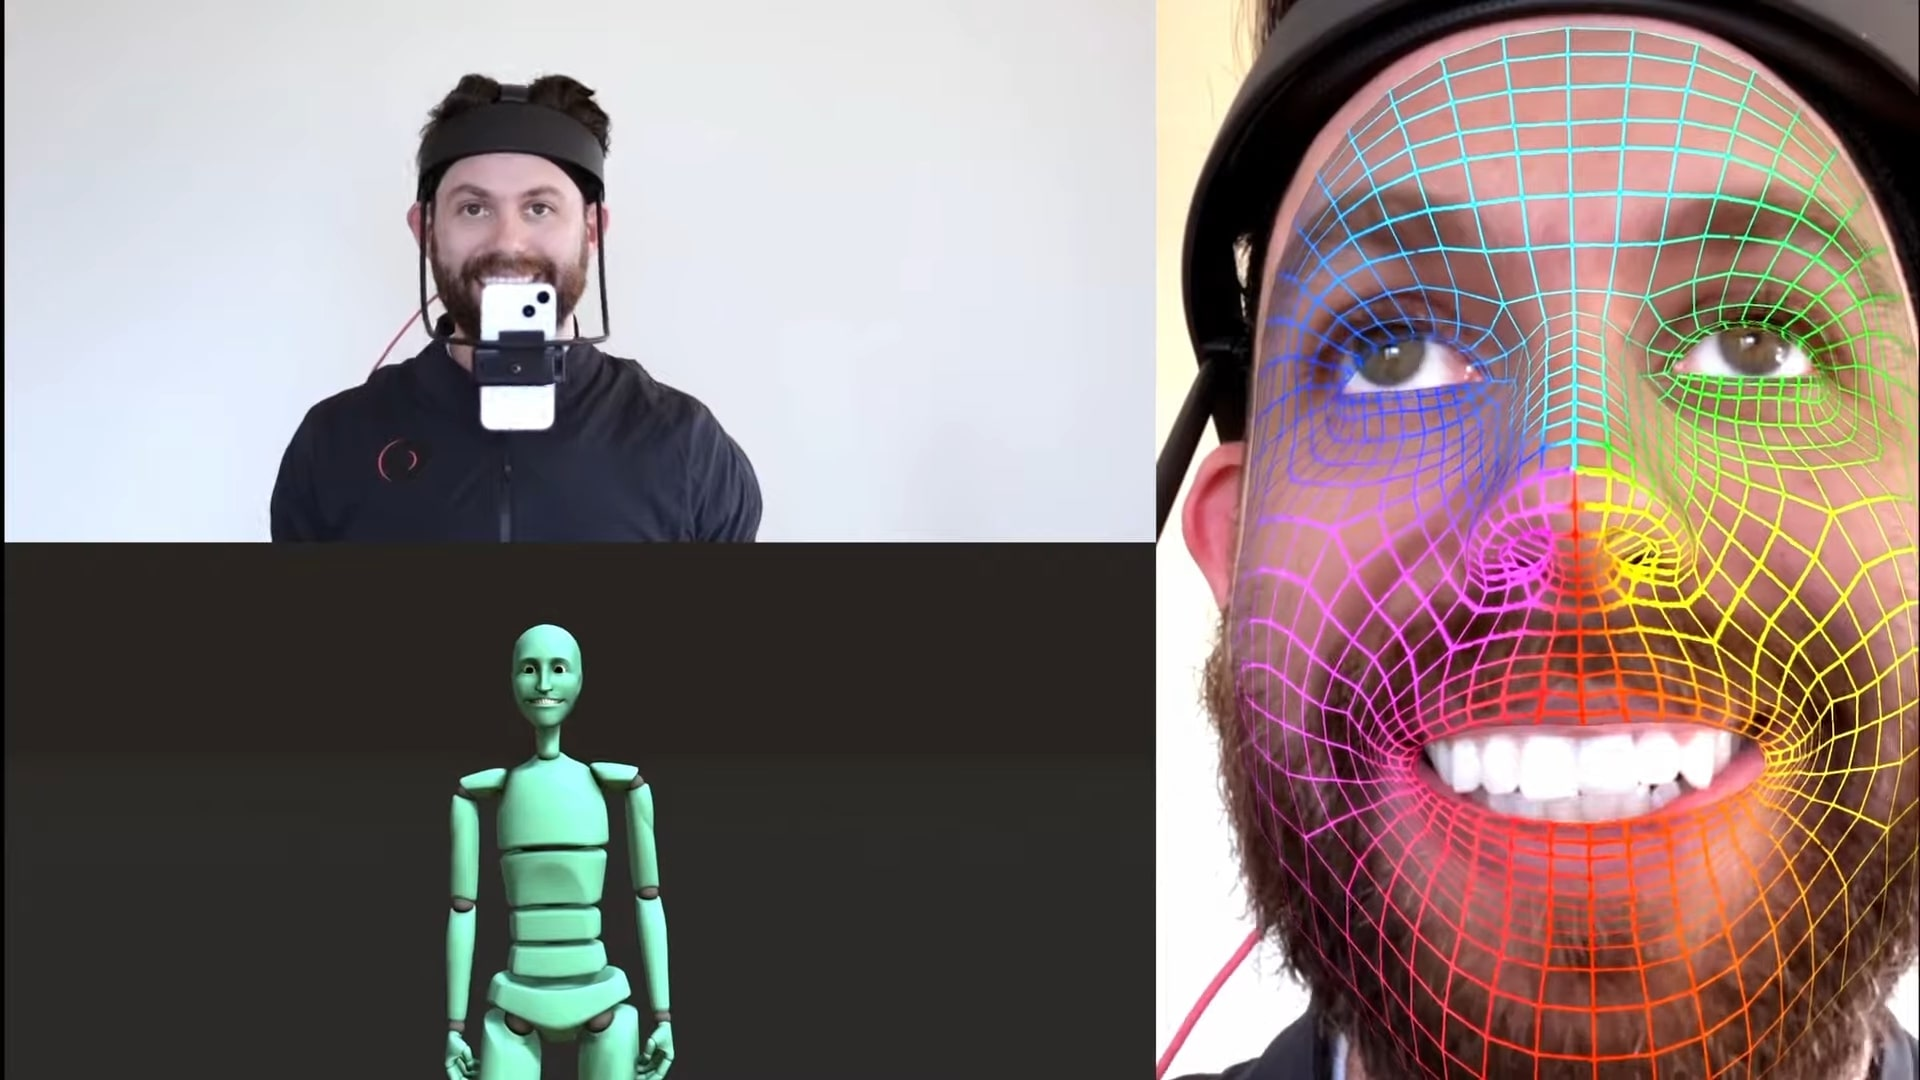
\includegraphics[width=0.8\textwidth]{chapters/facial_expressions/images/motion_capture.jpg}
    \caption{Performance-based facial animation using Apple's ARKit}
    \label{ch:facial_expressions:fig:motion_capture}
\end{figure}

todo fix face ex

todo fix intermediate inbetweeening


\section{Related Work}
\label{ch:intermediate_blocks_pose_correction:related_work}

In this section we will discuss the related work on AZee Templates, Motion Curves, and Motion Templates. 

\subsection{AZee Templates}
\label{ch:intermediate_blocks_pose_correction:related_work:azee_templates}

AZee templates are abstract representations used in \gls{sl} synthesis, linking linguistic descriptions with animated motions. For example, an AZee template like \texttt{:info-about(:car,?color)} could match an expression such as \texttt{:info-about(:car,:red)}, where the variable \texttt{color} would be assigned the value \texttt{:red}. This template instructs the avatar to convey information about a car's color, where the specific color (red, in this case) is dynamically inserted based on the template match. This approach allows for the dynamic generation of animations based on linguistic input, enabling avatars to respond to a wide range of queries and commands.

\subsection{Motion Curves}
\label{ch:intermediate_blocks_pose_correction:related_work:motion_curves}

Motion curves, (often refered as function curves or F-curves), have been extensively used in 3D character animation to control the timing and spacing of movements. These curves provide a graphical representation of a parameter's change over time, making them an essential tool in achieving realistic and fluid motion in animations(figure~\ref{fig:fcurves_blender}). Early foundational work by Witkin and Kass~\cite{witkin1988spacetime} introduced spacetime constraints, which used optimization techniques to control motion curves in generating realistic animations under physical constraints. This idea has evolved, and modern techniques now integrate deep learning models with motion curves to enhance control and automate the generation of complex animations.

In the context of Sign Language,~\cite{inproceedings} discuss the use of 3D motion analysis to accurately capture and animate \gls{sl} gestures by extracting motion curve parameters from sensors like Microsoft Kinect. These motion curves, which represent the trajectories of movements made during signing, are essential for animating virtual signers in a natural and precise manner. The paper highlights how these curves are mathematically defined, including their type, plane of motion, and velocity, which are then used to recreate realistic \gls{sl} animations, enhancing applications like \gls{sl} recognition and machine translation.

\begin{figure}
    \centering 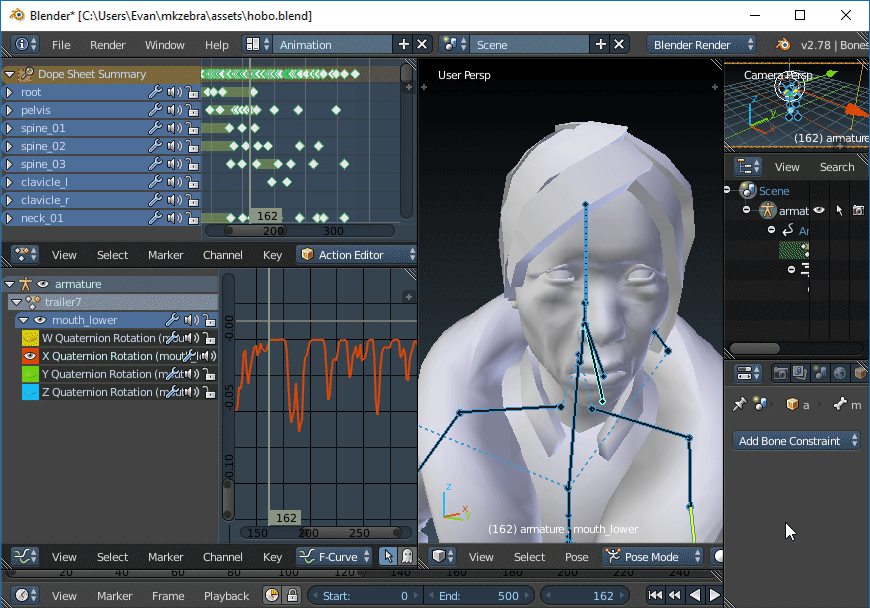
\includegraphics[width = 2.5in]{chapters/intermediate_blocks/images/fcurves_blender.png}
    \caption{F-curves in Blender}
    \label{fig:fcurves_blender}
\end{figure}

In recent research, deep learning methods have been employed to interpret and adapt motion curves for inbetweening tasks(figure~\ref{fig:inbetweening_transformers})~\cite{10.1145/3550454.3555454}. However, traditional mathematical optimization techniques are still widely in use. For example~\cite{10.1145/3306346.3322938} used tangent-space optimization to control character interpolations by allowing animators to directly manipulate positions and orientations, minimizing the need for additional keyframes. It ensures smooth transitions while respecting \gls{posture_constraint}s like joint limits and contact points, integrating seamlessly into existing animation workflows (figure~\ref{fig:inbetweening_disney}). 

\begin{figure}
    \centering \includegraphics[width = 2.5in]{chapters/intermediate_blocks/images/inbetweening_transformers.jpg}
    \caption{Motion Inbetweening using 2 stage Transformers~\cite{10.1145/3306346.3322938}}
    \label{fig:inbetweening_transformers}
\end{figure}

\begin{figure}
    \centering \includegraphics[width = 2.5in]{chapters/intermediate_blocks/images/inbetweening_disney.png}
    \caption{Rig Control using Tangent-Space Optimization}
    \label{fig:inbetweening_disney}
\end{figure}

\subsection{Motion Templates}
\label{ch:intermediate_blocks_pose_correction:related_work:motion_templates}

Motion templates offer a reusable framework for applying pre-defined motion patterns across different characters or scenarios. These templates are essentially built upon motion curves that define the motion's parameters, allowing for efficient replication and adaptation of complex motions. The concept of motion templates has been widely adopted in various fields, from character animation to robotic motion planning. Modern approaches often combine motion templates with machine learning techniques to facilitate the adaptation of these templates to new contexts, such as different character anatomies or environmental conditions.

In the context of character animation, motion templates can be particularly advantageous. The reusable nature of these templates allows for the consistent production of motion across different avatars while ensuring that the nuances of each motion are preserved. A method for controlling avatars using clustered motion segments from a large motion capture database was introduced by~\cite{10.1145/566654.566607}, enabling efficient real-time animation with intuitive user interfaces.

The Paula avatar uses AZee geometric templates that can be applied across various signing scenarios. For example, a rule such as place-prf(proform-vehicle, midssp) allows for the placement of a vehicle proform in the middle of the signing space(figure~\ref{fig:azee_template_example}). This method leverages a consistent geometric system, enabling the natural synthesis of movements without relying on a fixed set of points, which is crucial for capturing the variability and dynamism inherent in sign language. This approach however, generates animations by focusing solely on higher-level linguistic structures rather than low-level constraints.

\begin{figure}
    \centering \includegraphics[width = 2.5in]{chapters/intermediate_blocks/images/azee_template_example.png}
    \caption{AZee Templates used by the Paula avatar}
    \label{fig:azee_template_example}
\end{figure}

For our experiments, we will be mainly using the \emph{40 brèves}~\cite{challant2022first} corpus. The frequency of the AZee rules in this corpus can be seen in figure~\ref{fig:azee_rule_frequency}.

\begin{figure}
    \centering \includegraphics[width = 5in]{chapters/intermediate_blocks/images/azee_rule_frequency.png}
    \caption{Frequency of AZee rules in the \emph{40 brèves} corpus}
    \label{fig:azee_rule_frequency}
\end{figure}

todo fix intermediate intbetweening



\paragraph{Uncanny Valley}
\label{ch:background_work:sign_language_synthesis:3d_techniques:avatar_animation:uncanny_valley}

The Uncanny Valley is a concept in robotics and 3D animation that describes the discomfort or eeriness people feel when they encounter a humanoid figure that is very close to, but not quite, human-like. This phenomenon was first identified by roboticist Masahiro Mori in 1970.

As avatars become more realistic in appearance and movement, they initially become more appealing and relatable. However, there is a point at which the avatar becomes almost, but not perfectly, human-like, causing a sense of unease or revulsion in the observer. This dip in the graph of familiarity versus human likeness is known as the Uncanny Valley.

Figure~\ref{fig:uncanny_valley_graph} illustrates the Uncanny Valley effect, showing how an increase in human likeness can lead to a dip in emotional response before rising again as realism improves.

\begin{figure}
  \centering
  \includegraphics[width = 2.5in]{chapters/background_work/images/uncanny_valley_graph.png}
  \caption{Graph illustrating the Uncanny Valley effect}
  \label{fig:uncanny_valley_graph}
\end{figure}

The factors contributing to the Uncanny Valley effect often include:

\begin{itemize}
  \item \textbf{Facial Expressions}: Subtle imperfections in facial expressions, such as unnatural eye movements or lifeless smiles, can make the avatar appear creepy or unsettling.
  \item \textbf{Movement}: Non-human-like movements, jerky motions, or slight deviations from natural human motion can heighten the uncanny effect.
  \item \textbf{Texture and Skin Tone}: Inconsistent skin textures, overly smooth surfaces, or unrealistic lighting and shading can make an avatar appear artificial.
  \item \textbf{Eye Contact}: The eyes are critical in conveying emotions and life. Any deviation in eye movement, blink patterns, or focus can make an avatar look eerie.
\end{itemize}

Understanding and mitigating the Uncanny Valley effect is crucial for animators and developers aiming to create realistic and relatable avatars. One way to avoid the Uncanny Valley could be to use stylized avatars, which are intentionally designed to deviate from realism and have a unique aesthetic. Another approach is to keyframe more information in the animations themselves, ensuring that movements and expressions are as natural and lifelike as possible.

\subsubsection{\gls{sl} Synthesis Systems}
\label{ch:background_work:sign_language_synthesis:3d_techniques:sign_language_synthesis_systems}

In the context of \gls{sl} synthesis, several advanced systems have been developed to automate the generation and animation of sign language.

\paragraph{JASigning}
\label{ch:background_work:sign_language_synthesis:3d_techniques:sign_language_synthesis_systems:jasigning}

JASigning is an advanced \gls{sl} avatar system developed within the scope of the ViSiCAST and eSIGN projects. It enables the automatic generation and animation of \gls{sl} through a predefined set of gestures and animations. These gestures can be dynamically combined to form coherent \gls{sl} sentences. JASigning is designed to support multiple sign languages and integrates with text-to-sign translation systems. The system uses HamNoSys in the form of an XML representation to describe signs and their components. JASigning has been used in various applications, including educational tools, communication aids, and virtual avatars.

Figure~\ref{fig:jasigning} shows an example of the JASigning system in action.

\begin{figure} 
  \centering \includegraphics[width = 2.5in]{chapters/background_work/images/jasigning.png} 
  \caption{JASigning} 
  \label{fig:jasigning} 
\end{figure}

\paragraph{EMBR}
\label{ch:background_work:sign_language_synthesis:3d_techniques:sign_language_synthesis_systems:embr}

Unlike the previous models, EMBR (Embodied Agents Behaviour Realizer) Script is a scripting language used to control virtual characters in general and is not restricted to \gls{sl} avatars. However, EMBRScript allows for animation specification through a sequence of key poses, each defined at specific time points for a precise specification of body movements, facial expressions, and other actions. This also makes it usable to describe signs with synthesis using an avatar in mind.

EMBR is a real-time animation engine engineered to produce expressive gestures and \gls{sl} for virtual avatars. EMBR facilitates precise control over avatar movements, encompassing hand shapes, facial expressions, and body postures critical for accurate \gls{sl} depiction. The framework supports scripting and integrates with various input modalities, such as text or motion capture data, to generate realistic and contextually appropriate \gls{sl} animations. EMBR's flexibility and adaptability make it a valuable tool in research settings, particularly for studies focused on the nuances of non-verbal communication and the development of nuanced, context-sensitive gestures.

\paragraph{Synthesis based on Generative Models}
\label{ch:background_work:sign_language_synthesis:3d_techniques:sign_language_synthesis_systems:synthesis_based_on_generative_models}

Generative models have shown promise in \gls{sl} synthesis by learning the underlying structure of \gls{sl} data and generating new animations. These models can be trained on large datasets of \gls{sl} videos to capture the complex relationships between linguistic input and \gls{sl} output. Some popular generative models used in \gls{sl} synthesis include:

\subparagraph{Gloss based}
\label{ch:background_work:sign_language_synthesis:3d_techniques:sign_language_synthesis_systems:synthesis_based_on_generative_models:gloss_based}

\gls{sl} animation from text focuses on generating realistic \gls{sl} videos from written text. The process involves text-to-gloss conversion, gloss-to-pose generation, and pose-to-sign rendering. Recent approaches utilize neural networks and generative models to enhance animation fluidity and realism. One method uses dictionary examples and a codebook of signs to create continuous \gls{sl} sequences, incorporating both manual and non-manual features. However, challenges remain in annotating the data and training the models effectively, particularly in the production of natural hand and facial movements.

\subparagraph{SignAvatars}
\label{ch:background_work:sign_language_synthesis:3d_techniques:sign_language_synthesis_systems:synthesis_based_on_generative_models:signavatars}

The SignAvatars~\cite{yu2023signavatars} dataset introduces a large-scale, multi-prompt 3D \gls{sl} motion dataset with 70,000 videos and 8.34 million frames from 153 signers. It includes isolated and continuous signs, annotated with 3D meshes and biomechanically-valid poses. The dataset supports tasks such as 3D \gls{sl} recognition and production from text scripts, individual words, and HamNoSys notation. A novel annotation pipeline ensures accurate 3D holistic annotations. Evaluation metrics indicate significant improvements in generating natural and consistent 3D \gls{sl} animations from diverse textual inputs using models like Sign-VQVAE.

\subparagraph{Sgnify}
\label{ch:background_work:sign_language_synthesis:3d_techniques:sign_language_synthesis_systems:synthesis_based_on_generative_models:sgnify}

Recent advancements in 3D reconstruction from \gls{sl} (SL) videos~\cite{Forte_2023_CVPR}, focusing on isolated signs. SGNify leverages linguistic priors, such as hand-pose symmetry and invariance, to enhance the accuracy of hand-pose estimation in challenging \gls{sl} videos. The approach outperforms existing 3D body-pose estimation methods, particularly in handling self-occlusions and motion blur. Quantitative and perceptual evaluations demonstrate that SGNify's reconstructions are more natural and comprehensible than previous methods, achieving sign recognition rates comparable to original video performances.

\subsubsection{AZee based}
\label{ch:background_work:sign_language_synthesis:3d_techniques:sign_language_synthesis_systems:azee_based}

This subsection explores AZee-based \gls{sl} synthesis systems, highlighting advancements in avatar animation using both hierarchical modeling and low-level synthesis techniques.

\paragraph{Paula}
\label{ch:background_work:sign_language_synthesis:3d_techniques:sign_language_synthesis_systems:azee_based:paula}

The system extends the Paula avatar using AZee descriptions. AZee encodes both form and functional linguistic aspects, while Paula ensures smooth human motion. The approach leverages a hierarchical model to specify movements using larger linguistic structures, improving naturalness. Key innovations include embedding geometric \gls{posture_constraint}s and utilizing procedural techniques for dynamic, realistic animations. Proform placements are optimized by factoring semantic functions and applying common forms across multiple productions. This method addresses limitations in previous models, such as the lack of supporting torso motion and dynamic differences, leading to more fluid and expressive \gls{sl} animations.

\paragraph{Low-level synthesizer for AZee}
\label{ch:background_work:sign_language_synthesis:3d_techniques:sign_language_synthesis_systems:azee_based:low_level_synthesizer_for_azee}

This work presents a bottom-up (or low-level generation using constraint optimization) synthesis solution for the AZee system using off-the-shelf IK solvers. The approach (discussed in detail in~\ref{ch:multi_track}) generates procedurally computed animations from AZee's symbolic descriptions, leveraging Blender's 3D editor and iTaSC solver. This method handles \gls{posture_constraint}s as IK problems, translating skeletal poses into keyframes. Despite inherently robotic motion, it serves as a low-level fallback for the existing top-down system. Preliminary results show effective static pose generation and a trade-off between precision and computation time, enhancing the flexibility of \gls{sl} avatar systems by integrating procedural synthesis with predefined animations.

\section{Conclusion}
\label{ch:background_work:conclusion}

To summarize:

\begin{itemize} 
  \item Linear systems for \gls{sl} representation are limited in their expressive capacity and fail to capture the complexity of natural sign language.
  \item Non-linear systems provide better coverage and more accurately reflect the nuances of sign language.
  \item Systems like Paula and AZee, which incorporate both form and functional aspects, offer a promising approach but are hindered by the labor-intensive nature of hand-crafted animations.
  \item There is a need for low-level synthesis techniques to complement these high-level models, allowing for greater flexibility and coverage.
  \item Existing low-level synthesis approaches, such as those using IK solvers, provide a foundation but require further development to fully support the diverse requirements of \gls{sl} animation.
  \item By addressing these gaps, we aim to advance the state of \gls{sl} synthesis, making it more scalable and capable of generating natural and expressive animations.
\end{itemize}

Throughout this chapter, we have introduced, defined, and discussed a variety of concepts from three research areas that are key to this thesis: \textit{avatars}, \textit{\gls{sl} representation}, and \textit{\gls{sl} synthesis}. In the rest of the manuscript, we heavily rely on many of these concepts to investigate ways in which models for \gls{sl} synthesis can progressively learn and improve using newer techniques.

Therefore, in Chapter~\ref{ch:avatar_creation_pose_synthesis} and Chapter~\ref{ch:multi_track}, we study ways to create and rig a \gls{sl} avatar as well as Multi Track Timeline generation from AZee respectively. Chapter~\ref{ch:intermediate_blocks_pose_correction} dives deeper into reusing animations using template matching and newer deep learning models for synthesis. Additionally, the studies presented in Chapter~\ref{ch:facial_expresions} discuss means to synthesize facial expressions for \gls{sl} avatar. Lastly, Chapter~\ref{ch:conclusion} concludes the manuscript by summarizing the findings and discussing future research directions.

The background work specific to the various tasks and applications we address throughout the manuscript is presented and discussed in the corresponding chapters.
\end{document}
